\section{Results and Discussion}

In DISHTINY, cellular reproduction is contingent on resource collection and cellular decision-making (e.g., to execute the ``Reproduce'' instruction) and is not directly tied to the elapsing of updates.
So, although each replicate ran for the same number of updates, the number of cellular generations elapsed differs between replicates.
Indeed, because cellular reproduction is asynchronous, extant cells within a single replicate differ with respect to number of cellular generations removed from an initial seed cell.
However, computing the mean across extant cells for cellular generations elapsed at the end of a run provides a reasonable notion of phylogenetic depth.

\begin{table}
 \centering
 \begin{tabular}{l c|cc} % alignment of each column data
 \multicolumn{4}{c}{\textbf{Elapsed Cellular Generations}} \\
 & & \multicolumn{2}{c}{Resource Wave Size} \\
 & & Small & Large \\
 \hline
 \multirow{5}{*}{\STAB{\rotatebox[origin=c]{90}{\parbox{1.5cm}{\centering Mutational\\Load}}}} & 1 & $298 \pm 234$ & $50 \pm 38$ \\
 & 2 & $224 \pm 145$ & $32 \pm 10$ \\
 & 3 & $111 \pm 22$ & $17 \pm 3$
 \\
 & 4 & $74 \pm 11$ & $11 \pm 1$ \\
 & 5 & $120 \pm 2$ & $6 \pm 1$ \\
\end{tabular}
\caption{
Number of elapsed cellular generations by treatment (mean $\pm$ standard deviation across replicates).
}
\label{tab:cell_generations}
\end{table}


Table \ref{tab:cell_generations} shows mean cellular generations elapsed at the end of an evolutionary run for each treatment.
The number of elapsed cellular generations varies systematically across treatments, generally deceasing both with increasing mutational load and increased resource wave size.
Across treatments, elapsed cellular generation counts range from around 298 to around 6.

Large resource wave size may depress the cellular generation rate for two reasons.
Because of their reduced radius and duration, in our implementation small resource wave events occur more densely and more frequently.
Although each small resource wave dispenses less resource compared to large resource wave, the small resource wave replicates enjoy greater average resource availability per update.
In addition, forming the small same-channel groups required to fully exploit small resource waves is a less challenging task than forming the large same-channel groups required to fully exploit large resource waves.

There are also two reasons why mutational load may depress the cellular generation rate.
First, because mutations cause some proportion of reproduction events to result in dead offspring (e.g., offspring that execute an ``Apoptosis'' instruction) or sterile offspring (e.g., offspring that fail to execute the ``Reproduce'' instruction ), higher mutational load may inherently depress the growth rate of the population.
Second, higher mutational load may make developing and maintaining cooperative same-channel resource collection groups more difficult, therefore suppressing the resource collection rate.
For example, under greater mutational load same-channel resource collection groups may have to contend with members that unnecessarily expend resource replacing existing members with their offspring instead of growing the group, disrupt the group by inserting offspring with a new channel ID at the interior of the group, or hog resource that may otherwise be shared between group members.

\begin{figure}[!htbp]
\begin{center}
\rotatebox{90}{~~~~~Mutational Load 1}
\begin{subfigure}[b]{0.45\columnwidth}
  \centering
  Small Resource Wave\\~\\
  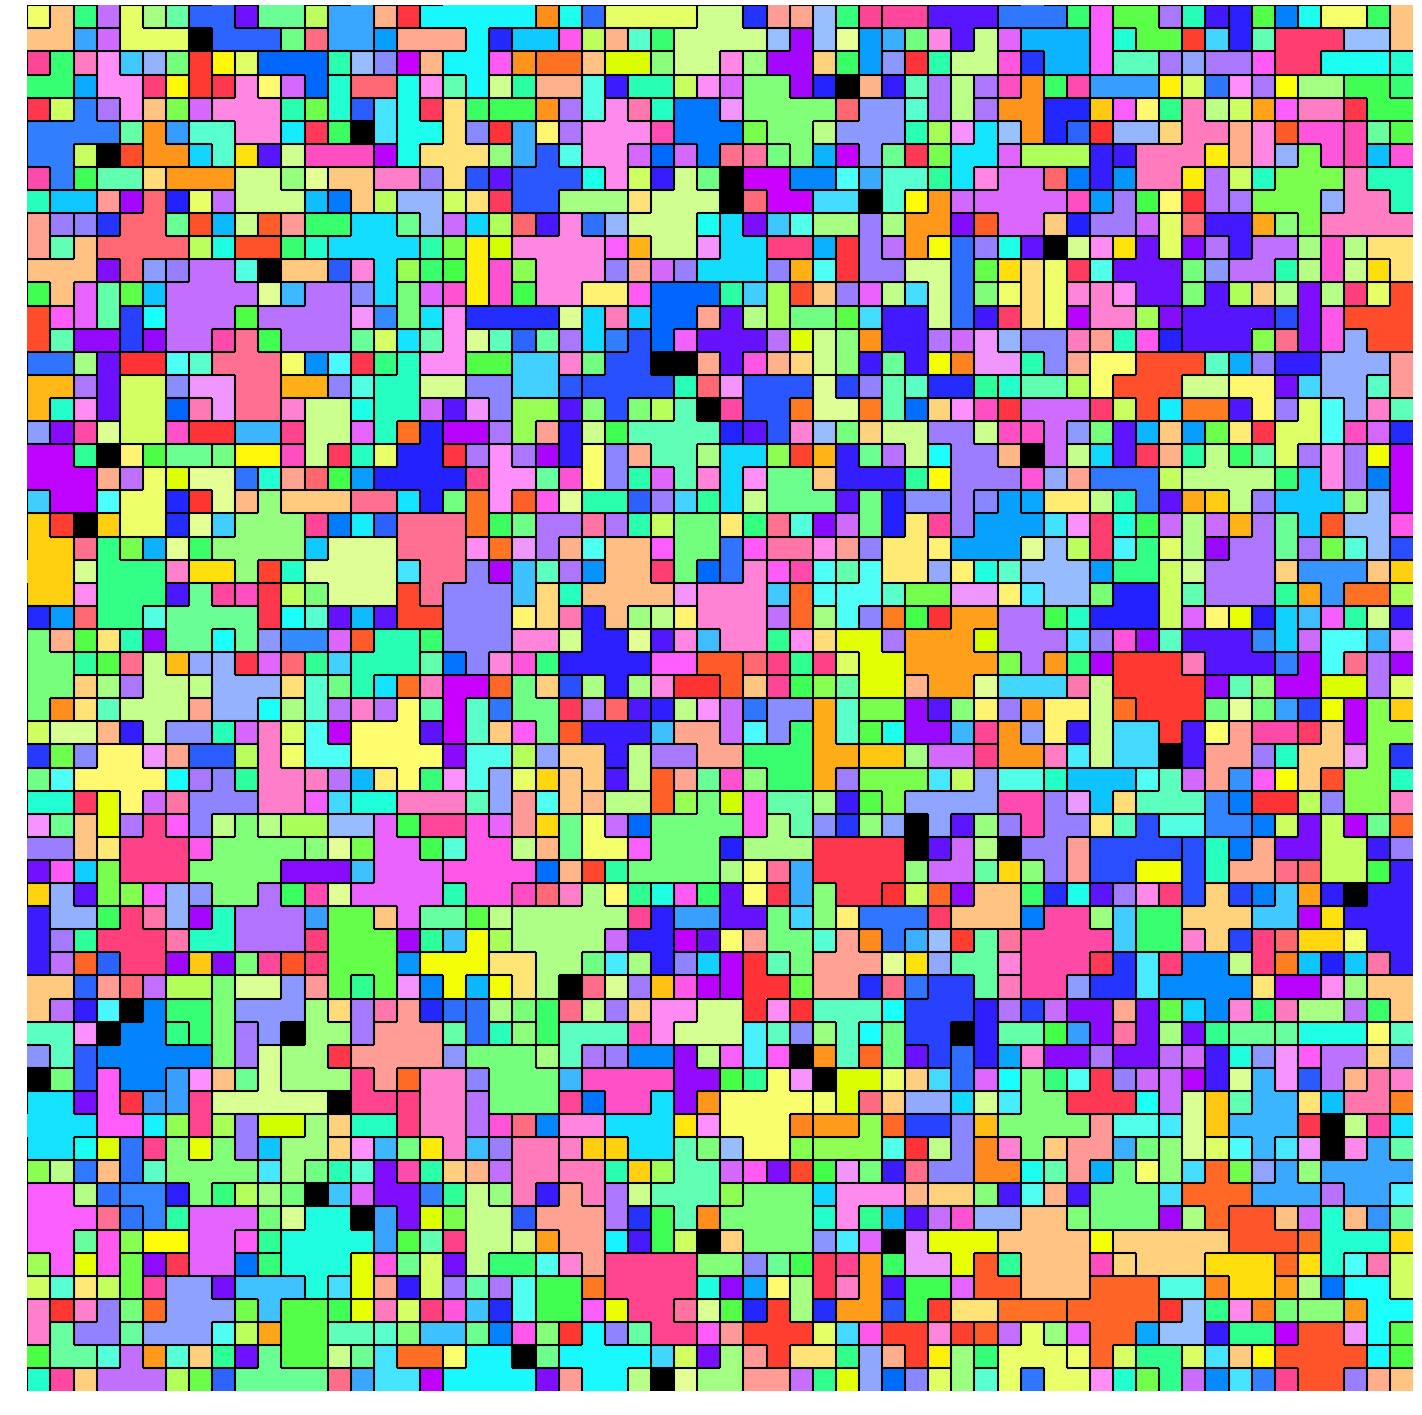
\includegraphics[width=\columnwidth]{seed=1001+title=channel_viz+treat=wave-small__mut-a_low+update=50000+_data_hathash_hash=38f284fb779ed3f5+_script_fullcat_hash=474b4115ecde8750+_source_hash=d53f428-clean+ext=}
\end{subfigure}
\begin{subfigure}[b]{0.45\columnwidth}
  \centering
  Large Resource Wave\\~\\
  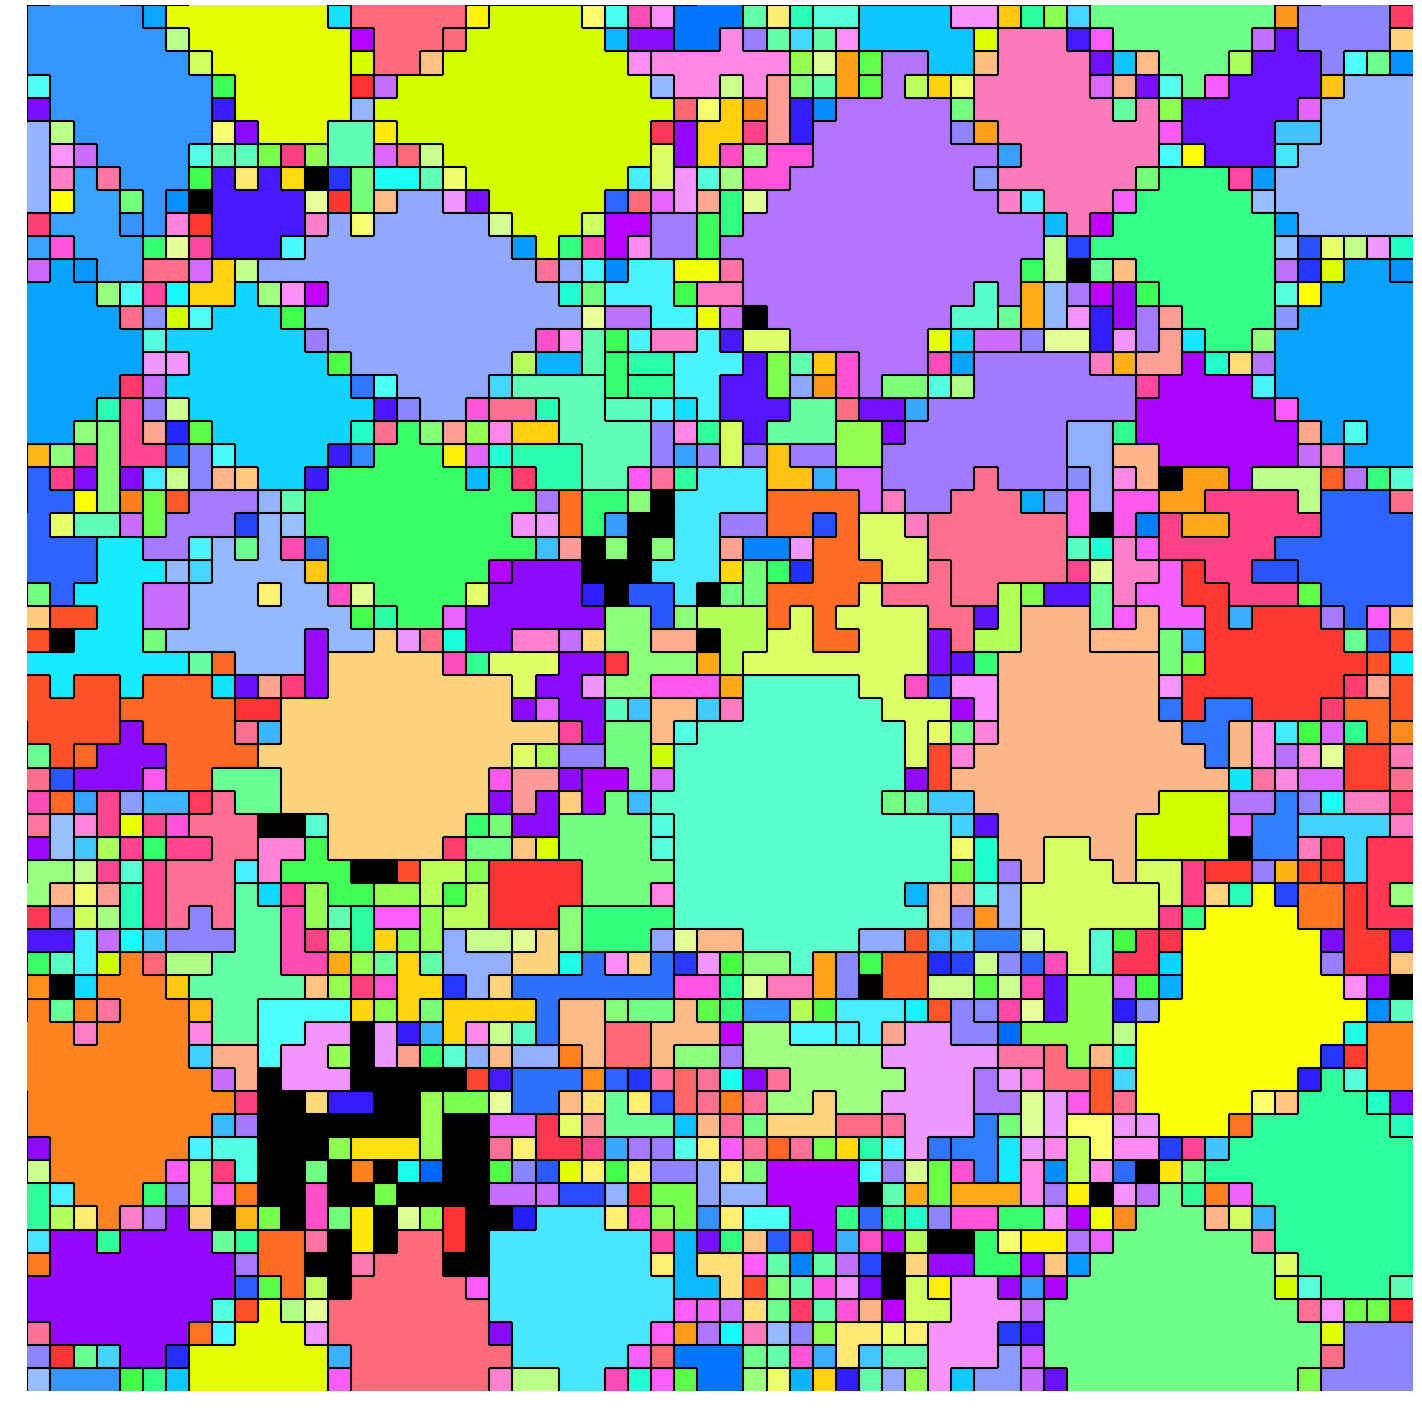
\includegraphics[width=\columnwidth]{seed=1001+title=channel_viz+treat=wave-big__mut-a_low+update=50000+_data_hathash_hash=33ac6f19e90e7ab9+_script_fullcat_hash=474b4115ecde8750+_source_hash=d53f428-clean+ext=}
\end{subfigure}

\rotatebox{90}{~~~~~~~Mutational Load 2}
\begin{subfigure}[b]{0.45\columnwidth}
  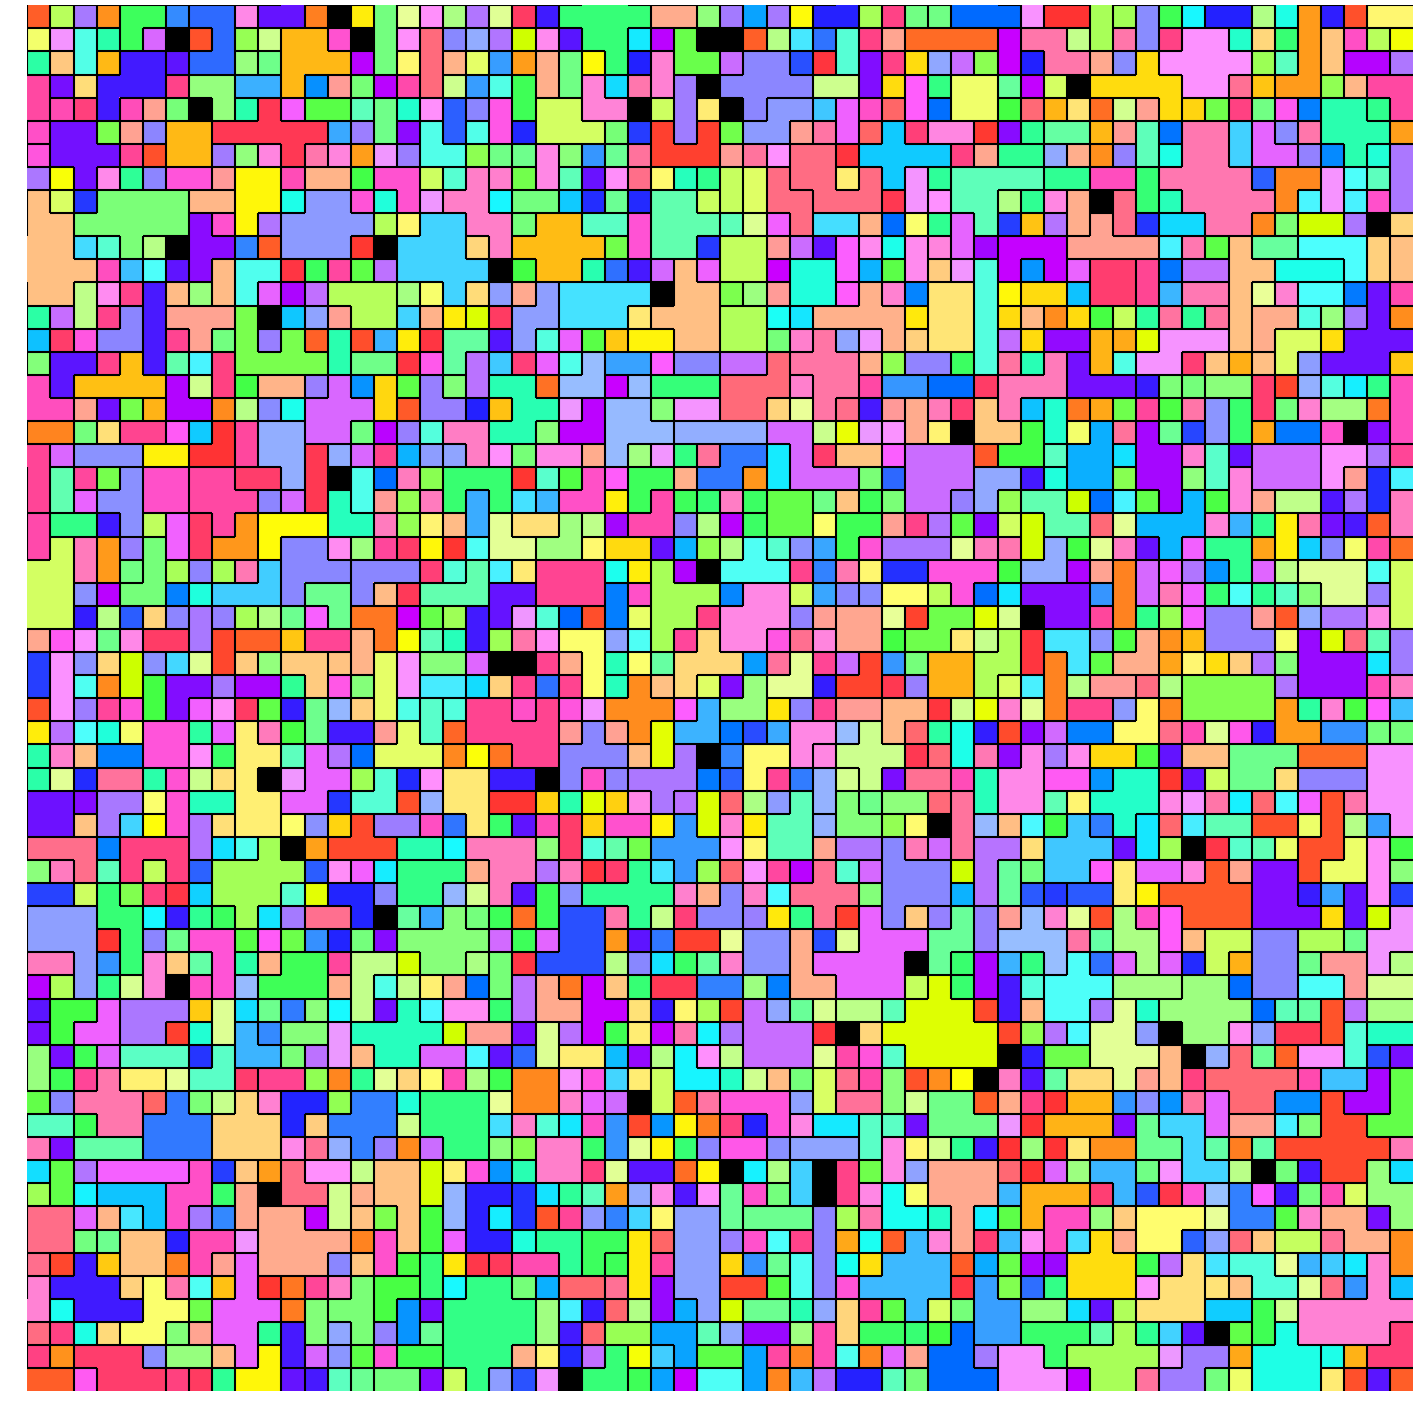
\includegraphics[width=\columnwidth]{seed=1001+title=channel_viz+treat=wave-small__mut-b_medlow+update=50000+_data_hathash_hash=0c0190afbbcd9acb+_script_fullcat_hash=474b4115ecde8750+_source_hash=d53f428-clean+ext=}
\end{subfigure}
\begin{subfigure}[b]{0.45\columnwidth}
  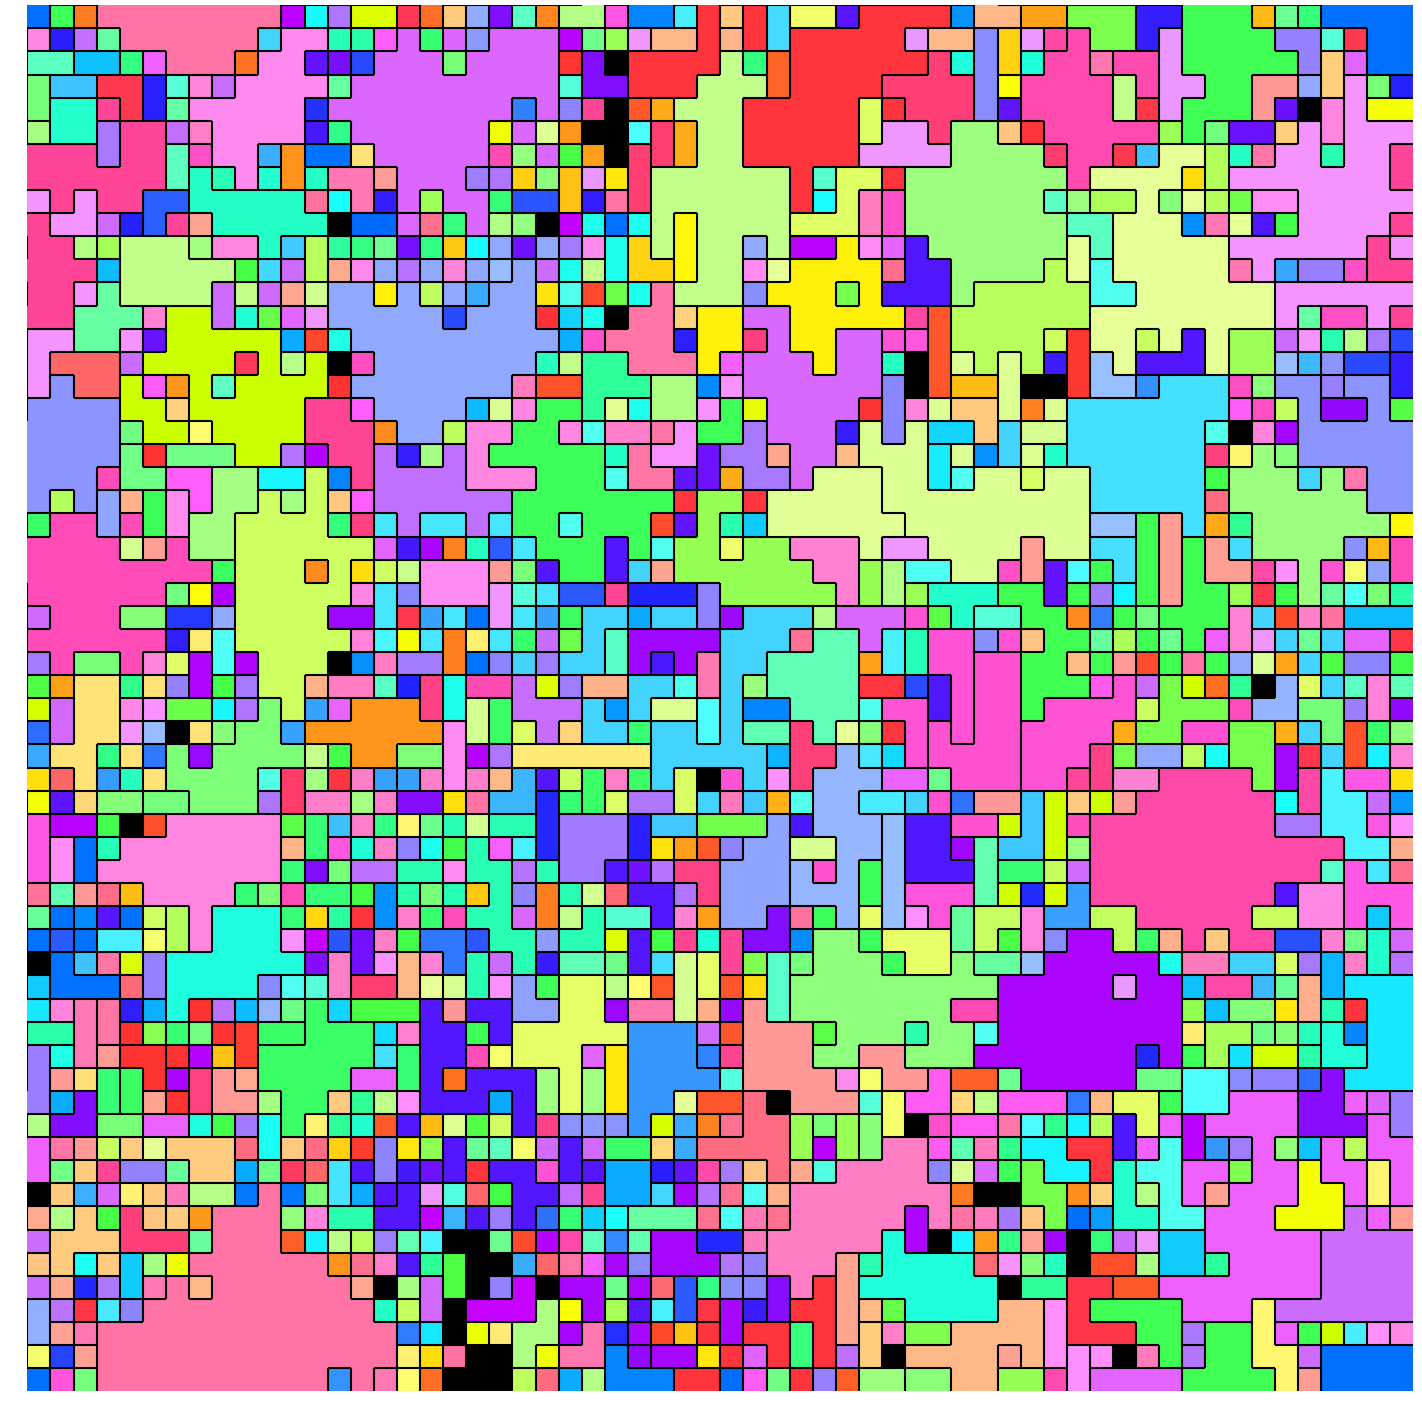
\includegraphics[width=\columnwidth]{seed=1001+title=channel_viz+treat=wave-big__mut-b_medlow+update=50000+_data_hathash_hash=50427fb0ffaf976a+_script_fullcat_hash=474b4115ecde8750+_source_hash=d53f428-clean+ext=}
\end{subfigure}

\rotatebox{90}{~~~~~~~Mutational Load 3}
\begin{subfigure}[b]{0.45\columnwidth}
  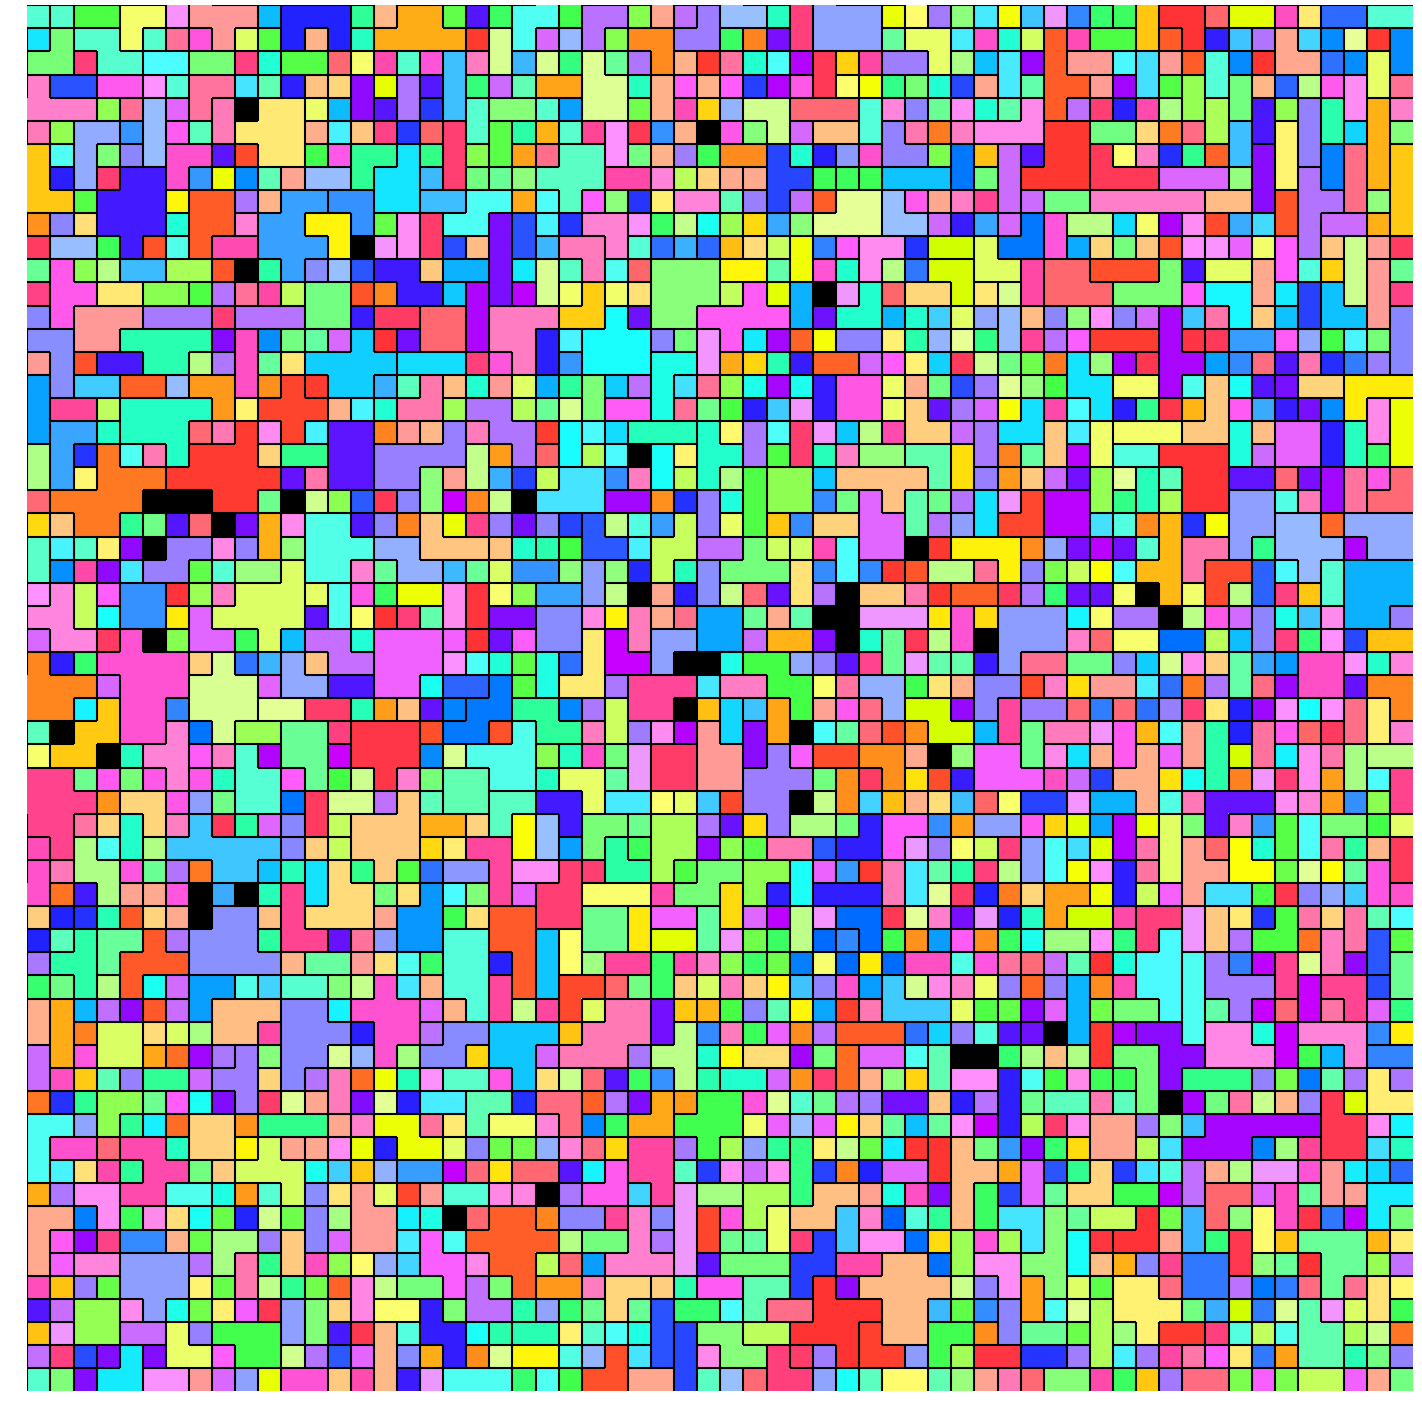
\includegraphics[width=\columnwidth]{seed=1001+title=channel_viz+treat=wave-small__mut-c_medhigh+update=50000+_data_hathash_hash=153e2f8791347e2b+_script_fullcat_hash=474b4115ecde8750+_source_hash=d53f428-clean+ext=}
\end{subfigure}
\begin{subfigure}[b]{0.45\columnwidth}
  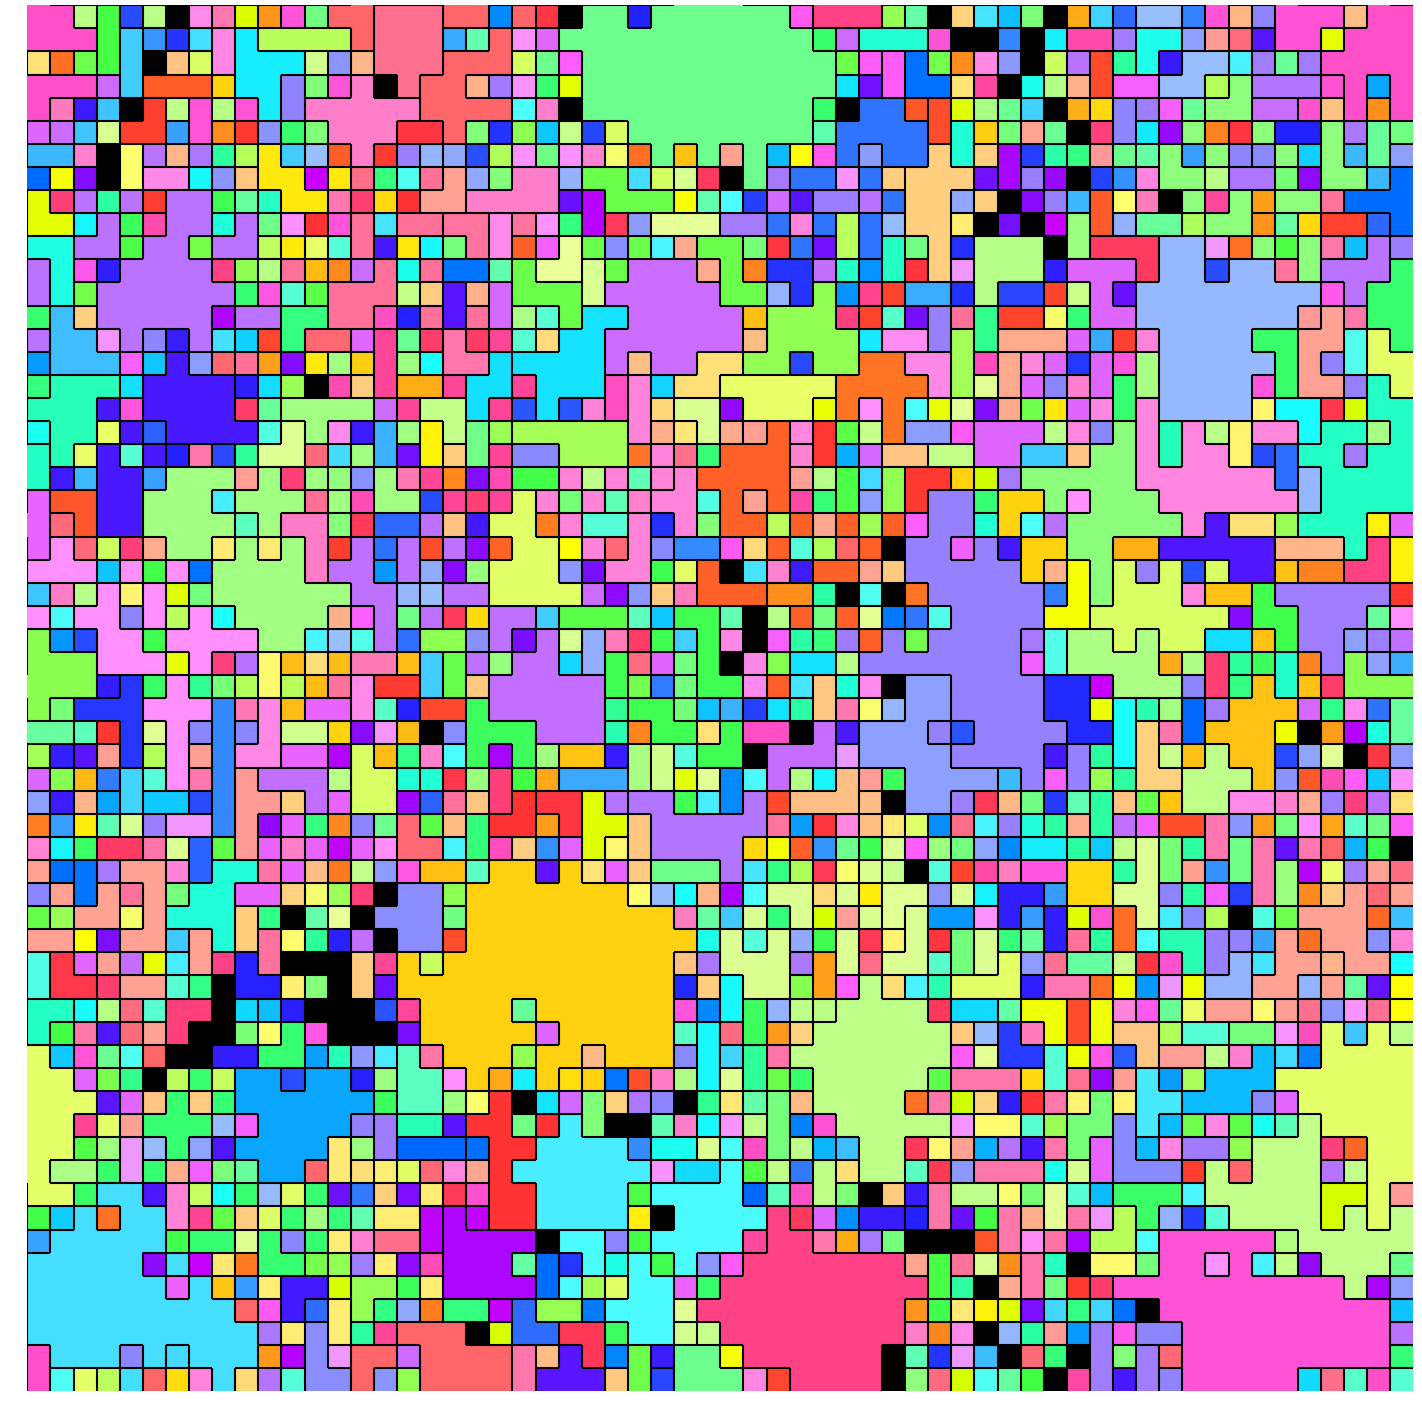
\includegraphics[width=\columnwidth]{seed=1001+title=channel_viz+treat=wave-big__mut-c_medhigh+update=50000+_data_hathash_hash=3bc8464cdb13317c+_script_fullcat_hash=474b4115ecde8750+_source_hash=d53f428-clean+ext=}
\end{subfigure}

\rotatebox{90}{~~~~~~~Mutational Load 4}
\begin{subfigure}[b]{0.45\columnwidth}
  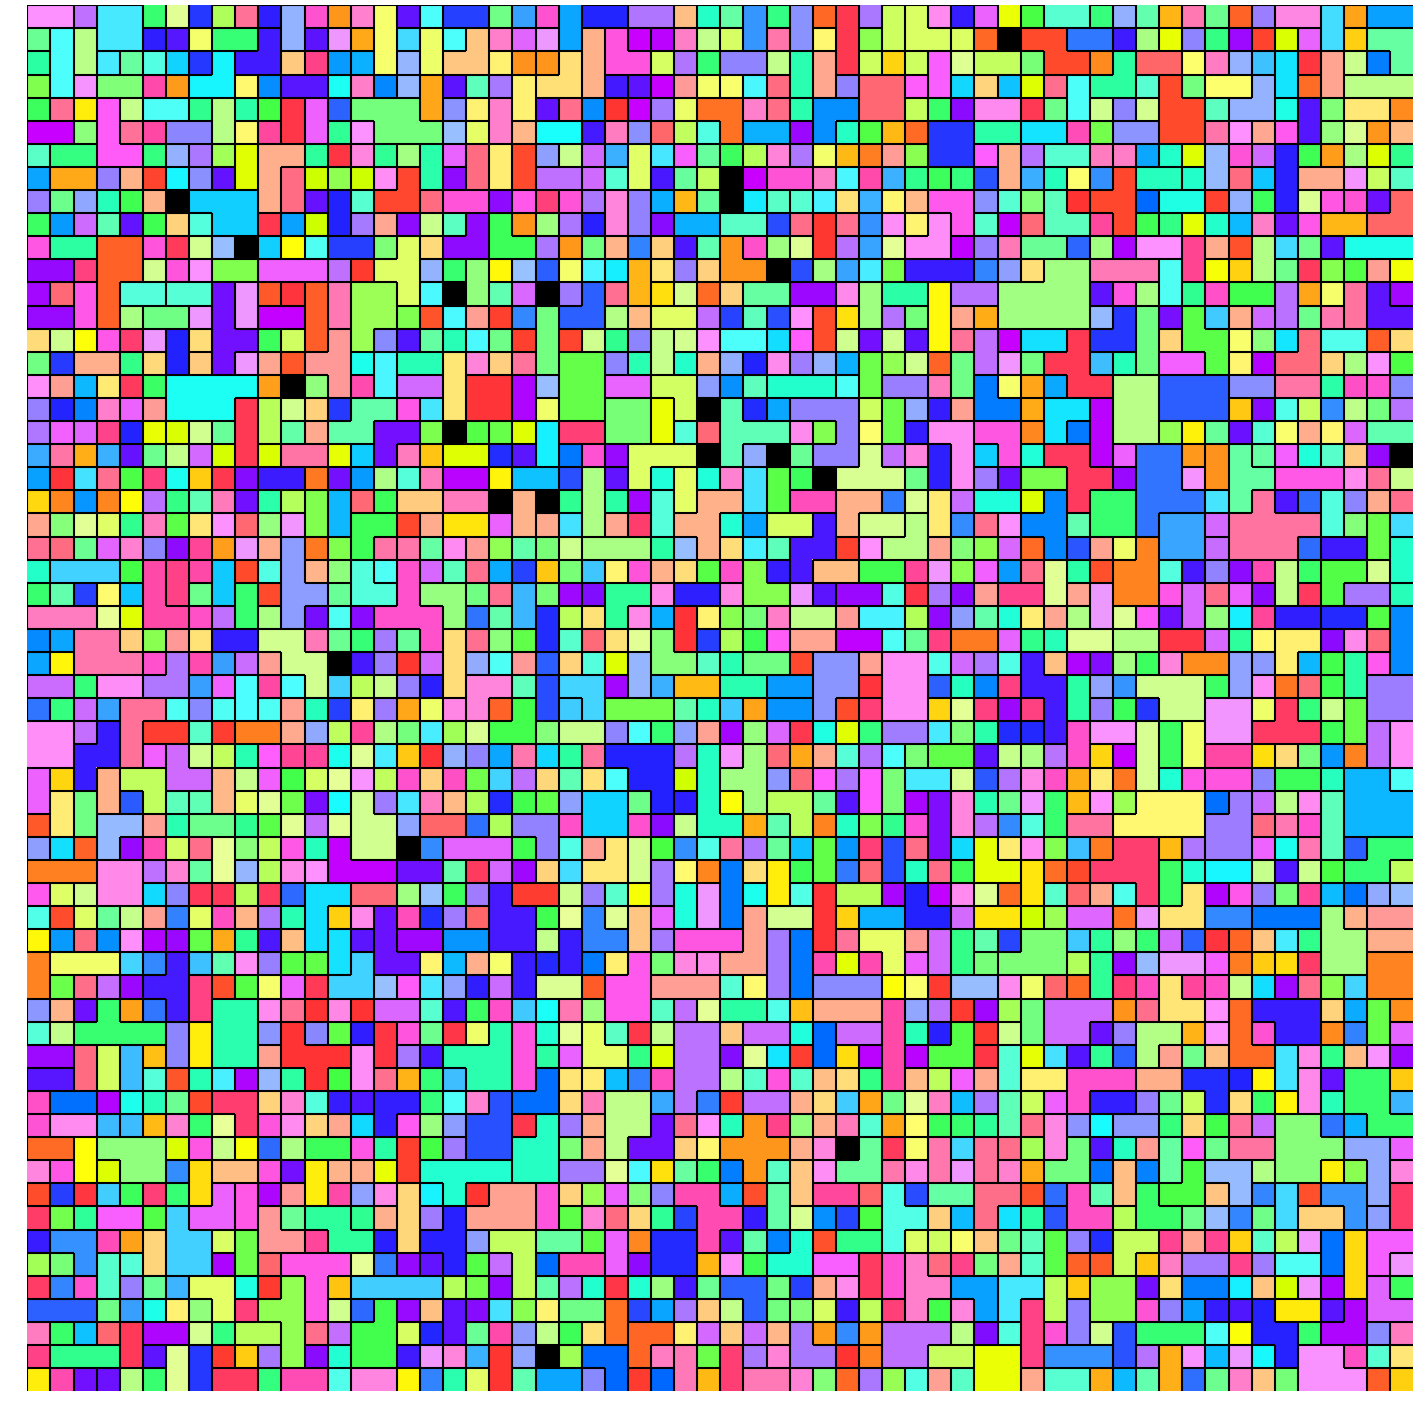
\includegraphics[width=\columnwidth]{seed=1001+title=channel_viz+treat=wave-small__mut-d_high+update=50000+_data_hathash_hash=700947e5ae80d046+_script_fullcat_hash=474b4115ecde8750+_source_hash=d53f428-clean+ext=}
\end{subfigure}
\begin{subfigure}[b]{0.45\columnwidth}
  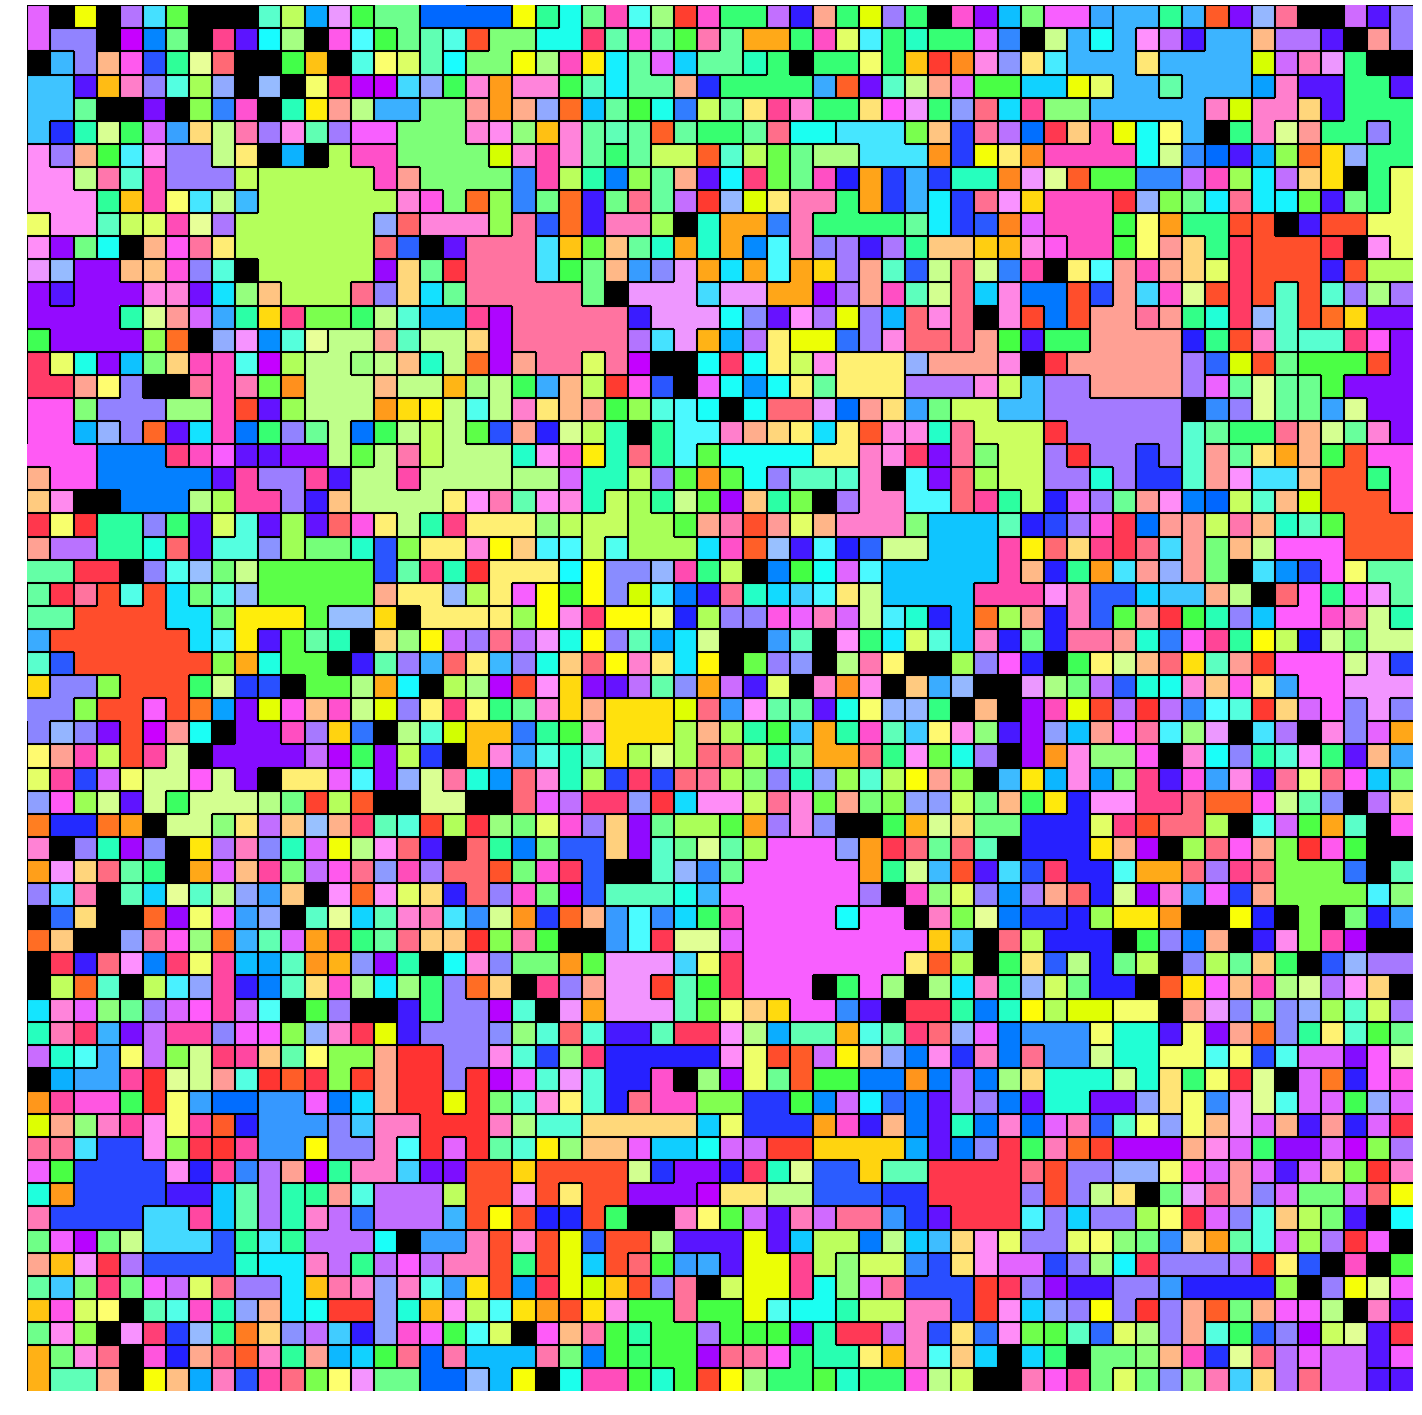
\includegraphics[width=\columnwidth]{seed=1001+title=channel_viz+treat=wave-big__mut-d_high+update=50000+_data_hathash_hash=e7071e390f076a00+_script_fullcat_hash=474b4115ecde8750+_source_hash=d53f428-clean+ext=}
\end{subfigure}

\rotatebox{90}{~~~~~~~Mutational Load 5}
\begin{subfigure}[b]{0.45\columnwidth}
  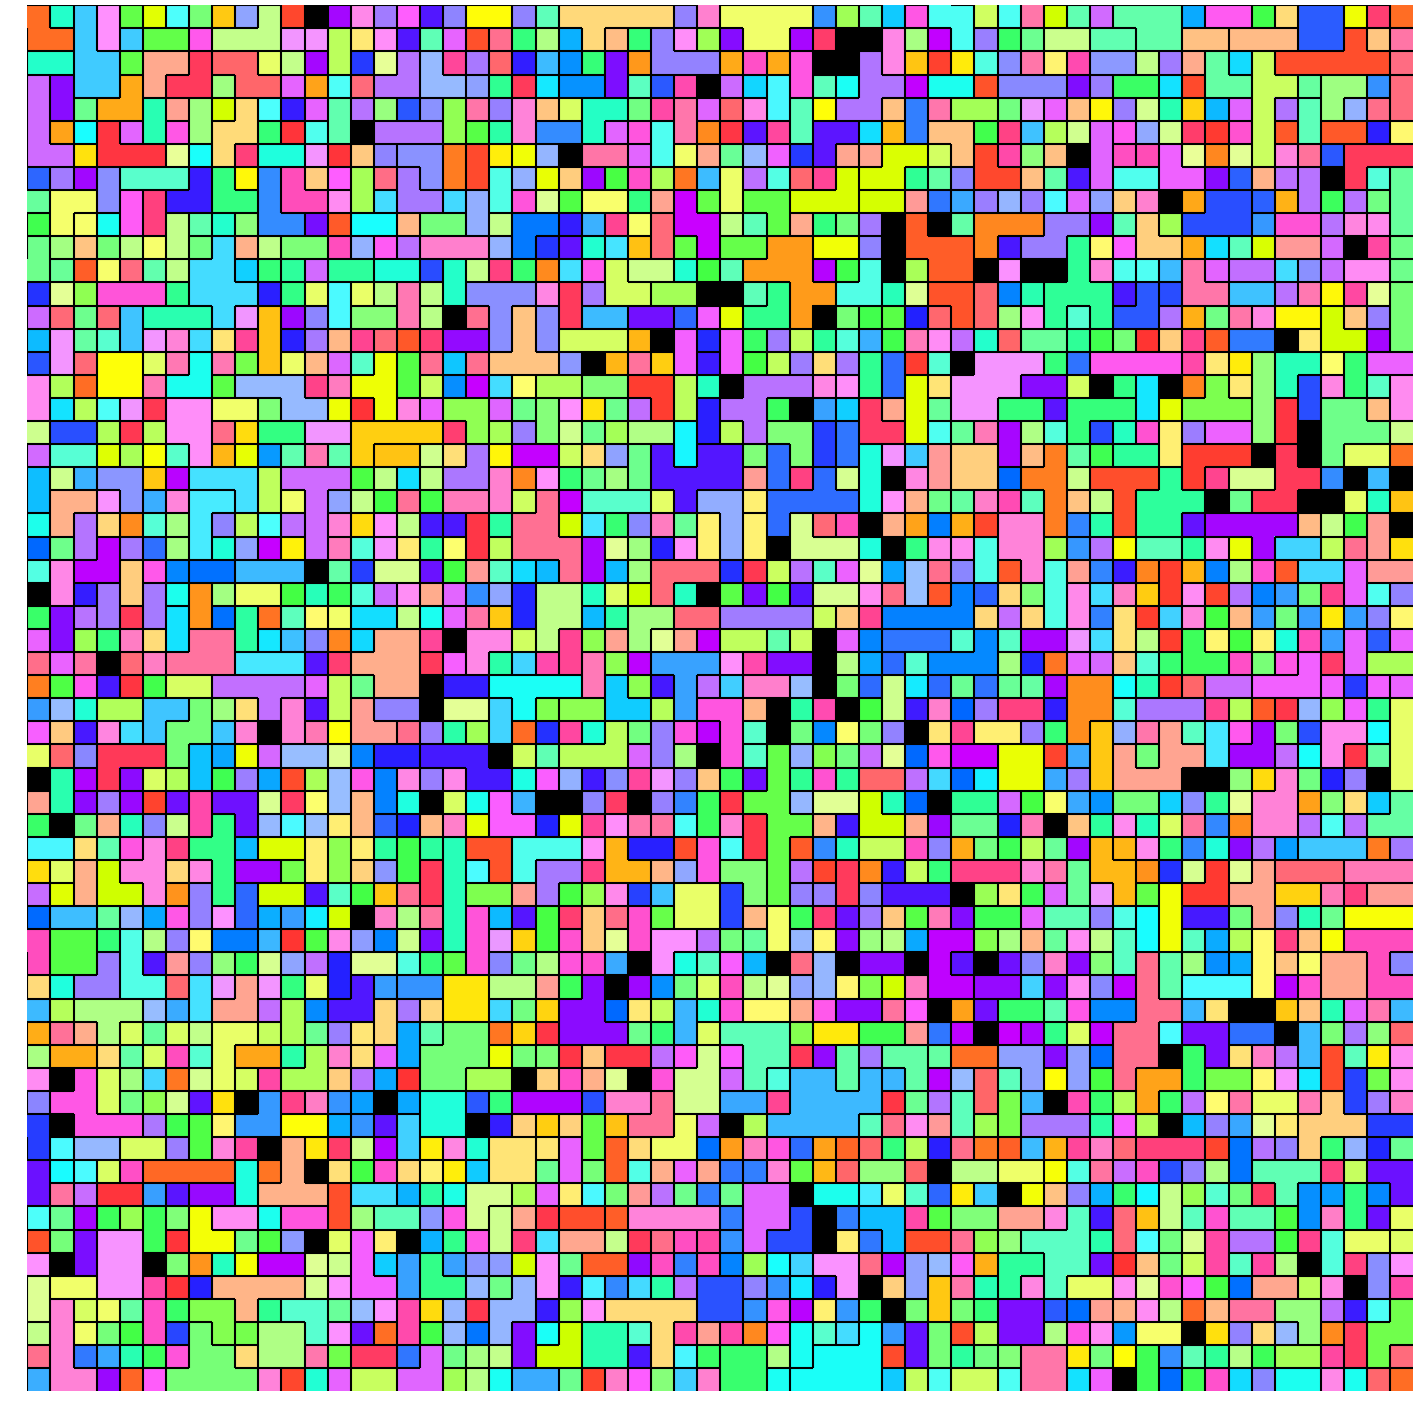
\includegraphics[width=\columnwidth]{seed=1001+title=channel_viz+treat=wave-small__mut-e_extreme+update=50000+_data_hathash_hash=70d59bcccb7f3ca6+_script_fullcat_hash=474b4115ecde8750+_source_hash=d53f428-clean+ext=}
\end{subfigure}
\begin{subfigure}[b]{0.45\columnwidth}
  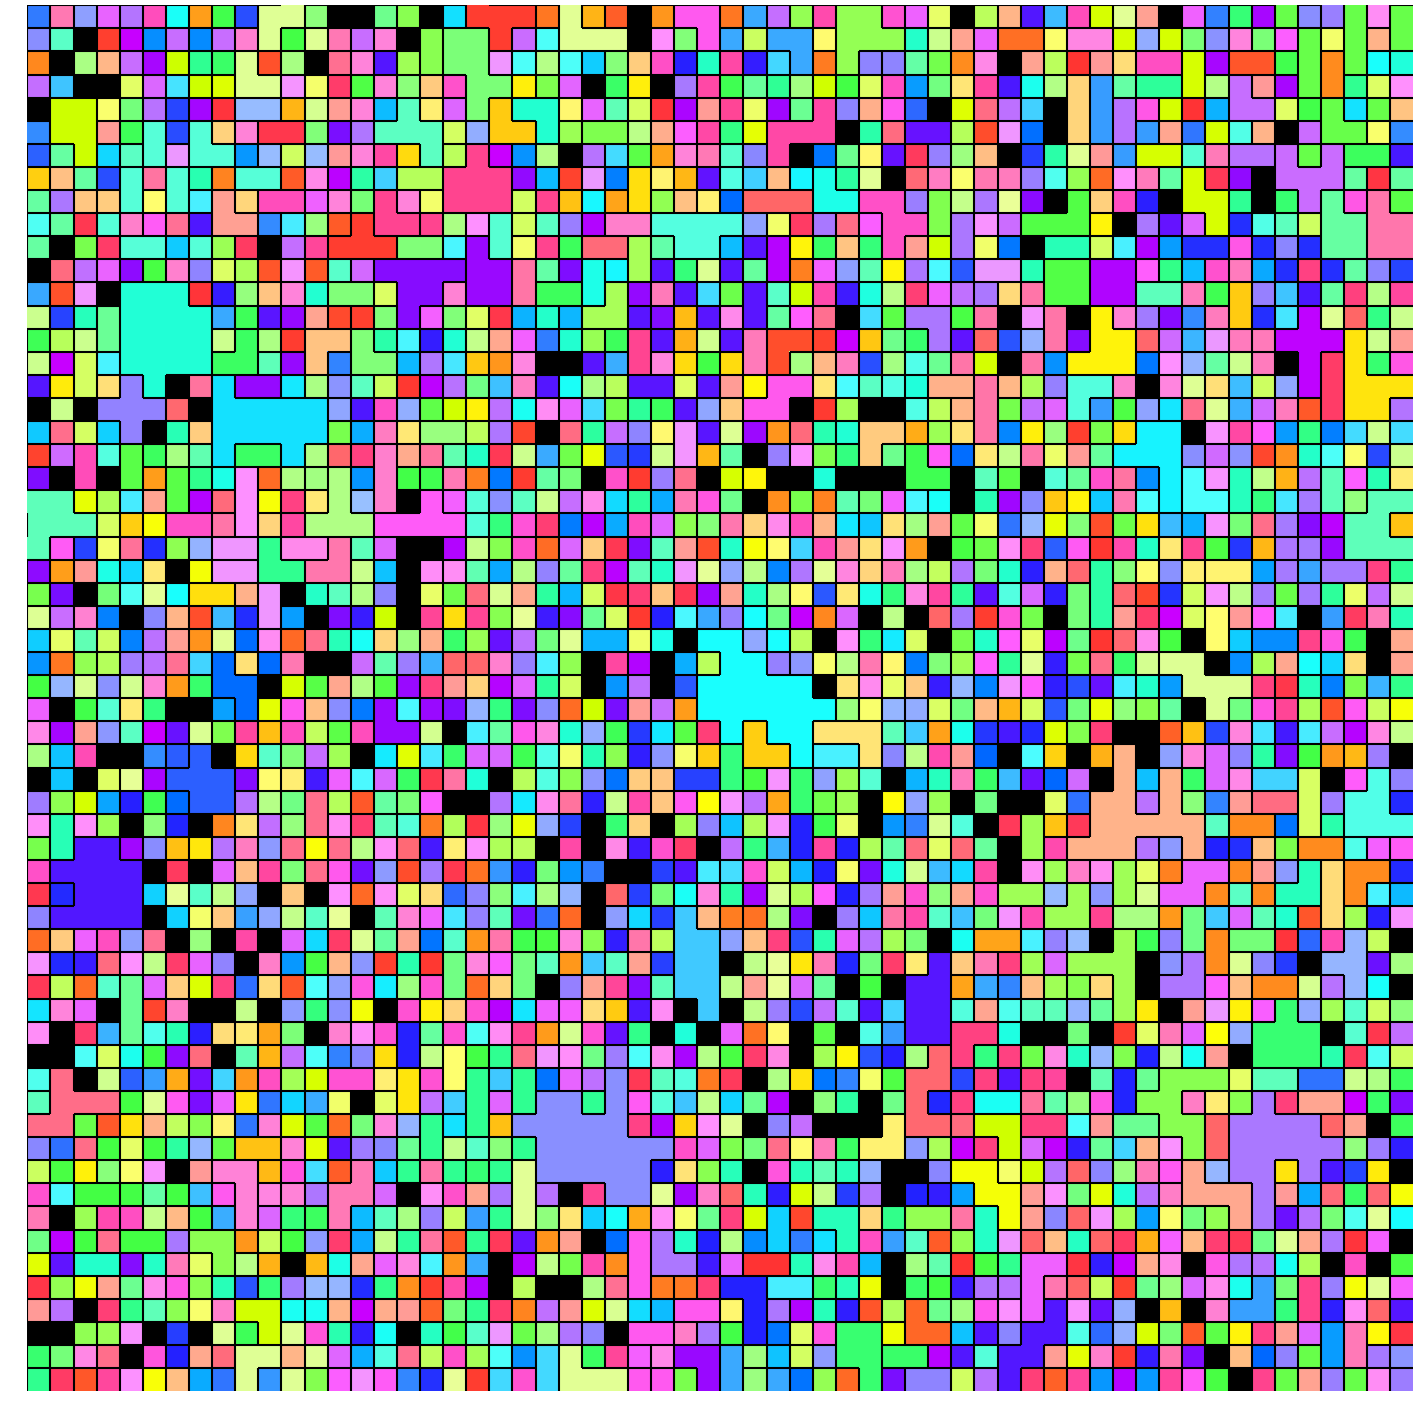
\includegraphics[width=\columnwidth]{seed=1001+title=channel_viz+treat=wave-big__mut-e_extreme+update=50000+_data_hathash_hash=6532b779898a7959+_script_fullcat_hash=474b4115ecde8750+_source_hash=d53f428-clean+ext=}
\end{subfigure}
\caption{
Representative same-channel signaling network end states for runs of each treatment.
A single cell-like organism occupies each grid tile except for black tiles, which are empty.
Channel IDs are coded by color.
Same-channel groups appear as uniformly-colored clumps, bounded by a black border.
}
\label{fig:outcome_grids}
\end{center}
\end{figure}


Indeed, in concordance with this second possibility, in Figure \ref{fig:outcome_grids} we can anecdotally observe more fragmented same-channel groups in treatments with greater mutational load.
This pattern is most strongly apparent in the large resource wave treatments, where the absence of large same-channel groups characteristic of low mutational load is easily observed under high mutational load, but also appears to hold for small resource wave treatments.
A more rigorous, quantitative analysis of this seeming pattern would benefit future work.

\begin{table}
 \centering
 \begin{tabular}{l c|cc} % alignment of each column data
 \multicolumn{4}{c}{\textbf{Extant Phylogenetic Roots}} \\
 & & \multicolumn{2}{c}{Resource Wave Size} \\
 & & Small & Large \\
 \hline
 \multirow{5}{*}{\STAB{\rotatebox[origin=c]{90}{\parbox{1.5cm}{\centering Mutational\\Load}}}} & 1 & $2 \pm 1$ & $61 \pm 52$ \\
 & 2 & $4 \pm 2$ & $80 \pm 51$\\
 & 3 & $5 \pm 1$ & $240 \pm 98$\\
 & 4 & $7 \pm 2$ & $599 \pm 82$\\
 & 5 & $28 \pm 3$ & $1204 \pm 116$\\
\end{tabular}
\caption{
Number of seed genomes with extant descendants (mean $\pm$ standard deviation across replicates).
}
\label{tab:phylogeny_roots}
\end{table}


The number of distinct phylogenetic roots among the extant population at the end of an evolutionary run provides a complimentary measure of evolutionary progress.
If only one phylogenetic root remains at the end of a run, the descendants of a single seeded cell have swept the entire population.
If two remain, the descendants of two distinct seeded cells are represented in the final population.
At the other end of the spectrum, 3600 phylogenetic roots would mean that a descendant from each and every seeded cell is present.
Table \ref{tab:phylogeny_roots} provides this metric for each treatment.
In agreement with Table \ref{tab:cell_generations}, the number of phylogenetic roots is lowest for low mutational load with small resource wave size (e.g., over more cellular generations, selection has eliminated a greater number of phylogenies) and the number of phylogenetic roots is greatest for high mutational load with large resource wave size (e.g., over fewer cellular generations, selection has yet to eliminate as many phylogenies).
From an evolutionary computing practitioner's perspective, the small number of extant phylogenies for low mutational load with small resource wave size --- generally, around two --- suggests that adaptive selection has strongly shaped the population in these replicates by the end of the evolutionary run.
However, the large number of extant phylogenies for high mutational load with large resource wave size --- generally, around 1200 --- suggests that adaptive selection has not as strongly shaped the population in these replicates by the end the of the evolutionary run.

With more computing time, we could extend the evolutionary runs of treatments with large resource wave size and/or larger mutational load in order to obtain populations with comparable evolutionary progress for all treatments.
However, we can still identify and discuss interesting differences between treatments while keeping this complicating factor in mind.

Now, we can turn to address the central question motivating this experiment: how does mutational load affect the evolutionary viability of cooperative strategies characteristic of fraternal transitions in individuality?
We're interested in two cooperative behaviors in particular,
\begin{itemize}
\item resource sharing between same-channel cells
\item and reproductive coordination between same-channel cells (e.g., cells reproducing over other-channel neighbors instead of same-channel neighbors).
\end{itemize}
Let's consider the effect of mutational load on each of these phenotypes in turn.

\begin{figure}[!t]
\begin{center}

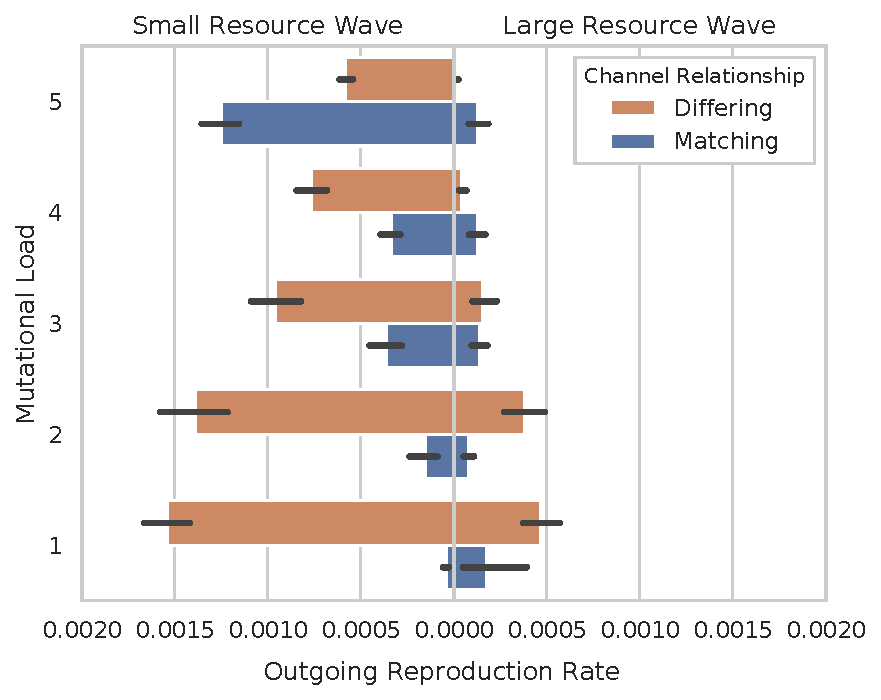
\includegraphics[width=\columnwidth]{title=reproductive_labor+_data_hathash_hash=4a000b28acccbd08+_script_fullcat_hash=970b6aa9f7815573+_source_hash=d53f428-clean+ext=}

\caption{
Reproductive cooperation phenotypes by treatment.
Small resource wave treatments are plotted on the left half of the plot, facing leftwards.
Large resource wave treatments are plotted on the right half of the plot, facing rightwards.
Mutational load increases in the upwards direction.
Bar height represents the mean per-update rate at which cells reproduce and replace a neighbor with their daughter cell, killing that neighbor.
Each two-tone pair of bars compares this rate with respect to neighbor cells that have matching channel ID and neighbor cell that do not.
Orange bars represent the rate at which cells reproduce over different-channel neighbors and blue bars represent the rate at which cells reproduce over same-channel neighbors.
Error bars represent 95\% confidence intervals.
The net outgoing reproduction rate (e.g., the sum height of bar pairs) differs by treatment because the net resource harvest rate, and therefore net cellular reproduction rate, depends on channel group configuration.
} \label{fig:reproductive_labor}
\end{center}
\end{figure}


Figure \ref{fig:reproductive_labor} compares reproductive cooperation phenotypes by treatment.
Under mutational load levels one and two in all treatments, cells preferentially reproduce over other-channel neighbors instead of same-channel neighbors ($p < 0.05$; bootstrap tests).
This observation matches expectation: same-channel groups that cooperate compete more efficiently for space than those that do not.
At mutational load levels three and four for small resource wave treatments, cells still preferentially reproduce over other-channel neighbors instead of same-channel neighbors ($p < 0.05$; non-overlapping 95\% confidence intervals).
However, at mutational load level three in large resource wave treatments this cooperative reproduction phenotype fades under large resource wave conditions.
In small resource wave treatments, the cooperative reproduction phenotype only disappears at the highest mutational load level, five.
Reproductive cooperation appears more robust to mutational load in small resource wave conditions than in large resource wave conditions.
This might be because this particular cooperative behavior is more essential to resource-collecting group formation and maintenance in smaller groups or because, due to the numerically smaller cell count of same-channel groups under the small wave treatment, the probability of dangerous mutant defectors (i.e., mutants that reproduce over same-channel neighbors) is smaller.

Surprisingly, at high mutational loads we actually observe active reproductive \textit{antagonism} between same-channel cells.
That is, cells preferentially reproduce over same-channel neighbors instead of other-channel neighbors.
This antagonistic phenotype occurs at mutational loads 4 and 5 under large resource wave conditions and at mutational load 5 under small resource wave conditions ($p < 0.01$; bootstrap tests).
A possible explanation of this surprising explanation is that under higher mutational loads when the behavior of same-channel kin is more uncertain these kin actually pose a greater threat to a cell than other-channel neighbors.
Because resource collection rate depends on same-channel group configuration, if a cell has collected enough resource to reproduce it is likely that its same-channel kin are also capable of reproducing.
Hence, cells would choose to antagonistically reproduce over same-channel kin to eliminate them (instead of eliminating other-channel neighbors, which are perhaps less likely to have enough resource to pose a reproductive threat).
Further study would be required to evaluate this hypothesis.

\begin{figure}[!htbp]
\begin{center}

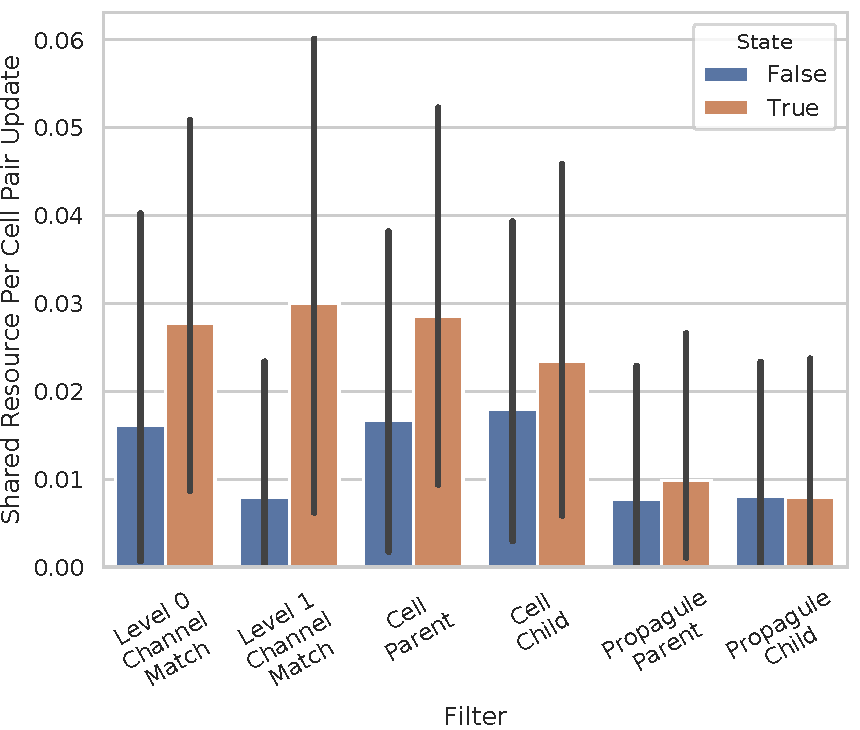
\includegraphics[width=\columnwidth]{script_hash=TODO_source_hash=TODO_emp_hash=TODO+treat=resource-wave__channelsense-yes__nlev-two+title=resource_contributed}
\caption{
TODO
}
\label{fig:resource_contributed}
\end{center}
\end{figure}


Figure \ref{fig:resource_contributed} compares resource sharing phenotypes under different treatments.
Under low mutational load (levels one and two), cells in large and small resource wave treatments preferentially share resource with same-channel neighbors ($p < 0.05$; bootstrap test).
At mutational load levels three and above, resource sharing rates decline sharply among cells in small resource wave treatments and cells do not preferentially share resource with same-channel neighbors ($p = 0.27, 0.43, 0.43$; bootstrap test).
At mutational load level three in large resource wave treatments, however, cells continue to preferentially share resource with same-channel neighbors ($p < 0.05$; bootstrap test).
At mutational load levels four and five, in large resource wave treatments cells actually preferentially share resource with neighbors with \textit{different} channel ID ($p < 0.0001$; bootstap test).

\begin{sidewaysfigure*}
\begin{center}
\rotatebox{90}{~~~~~~Small Resource Wave}
\hspace{1ex}
\begin{subfigure}[b]{0.1825\linewidth}
  \centering
  Mutational Load 1\\~\\
  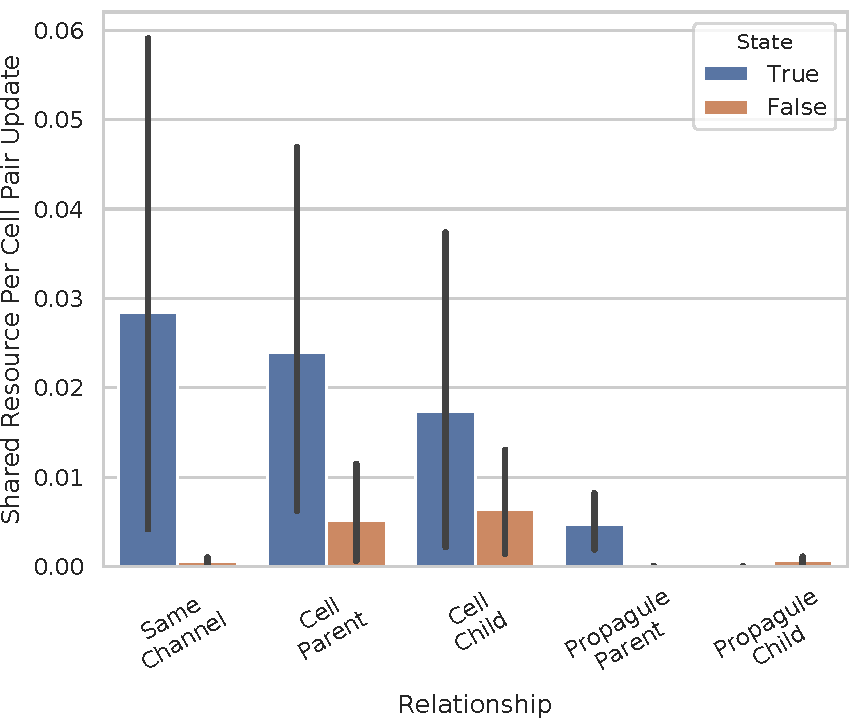
\includegraphics[width=\linewidth]{title=resource_contributed+treat=wave-small__mut-a_low+_data_hathash_hash=e071a43082c10cd4+_script_fullcat_hash=064800f3ddff6753+_source_hash=d53f428-clean+ext=}
\end{subfigure}
\hspace{1ex}
\begin{subfigure}[b]{0.1825\linewidth}
  \centering
  Mutational Load 2\\~\\
  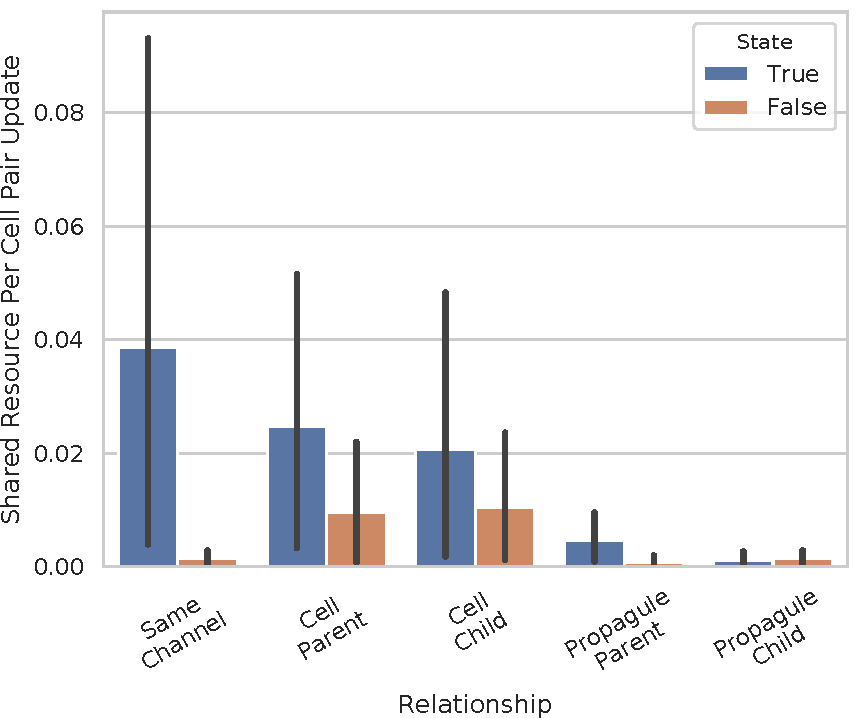
\includegraphics[width=\linewidth]{title=resource_contributed+treat=wave-small__mut-b_medlow+_data_hathash_hash=b470f6e885f49798+_script_fullcat_hash=064800f3ddff6753+_source_hash=d53f428-clean+ext=}
\end{subfigure}
\hspace{1ex}
\begin{subfigure}[b]{0.1825\linewidth}
  \centering
  Mutational Load 3\\~\\
  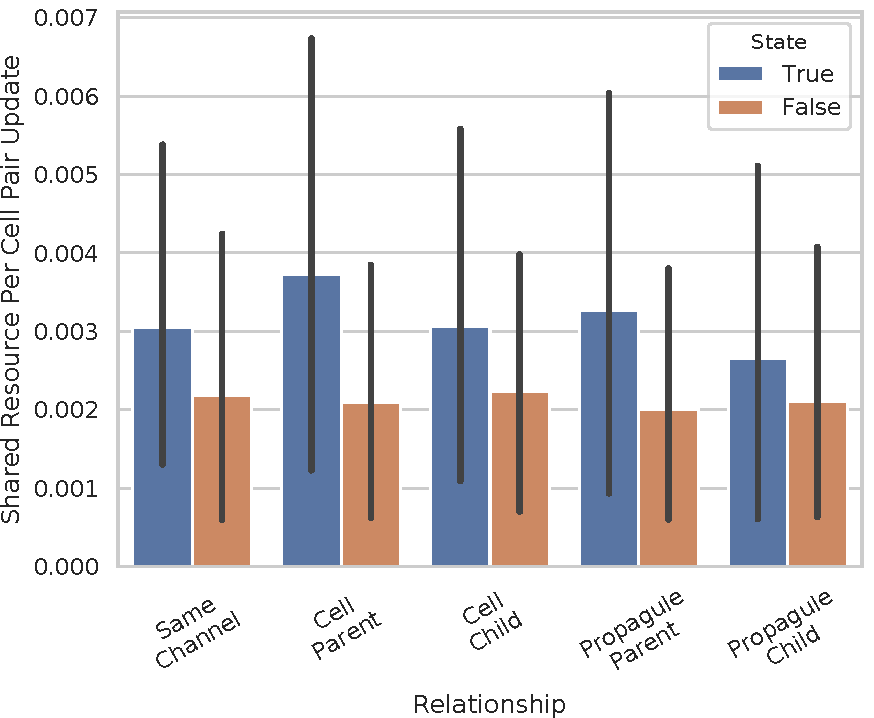
\includegraphics[width=\linewidth]{title=resource_contributed+treat=wave-small__mut-c_medhigh+_data_hathash_hash=09904fe0c4f292cc+_script_fullcat_hash=064800f3ddff6753+_source_hash=d53f428-clean+ext=}
\end{subfigure}
\hspace{1ex}
\begin{subfigure}[b]{0.1825\linewidth}
  \centering
  Mutational Load 4\\~\\
  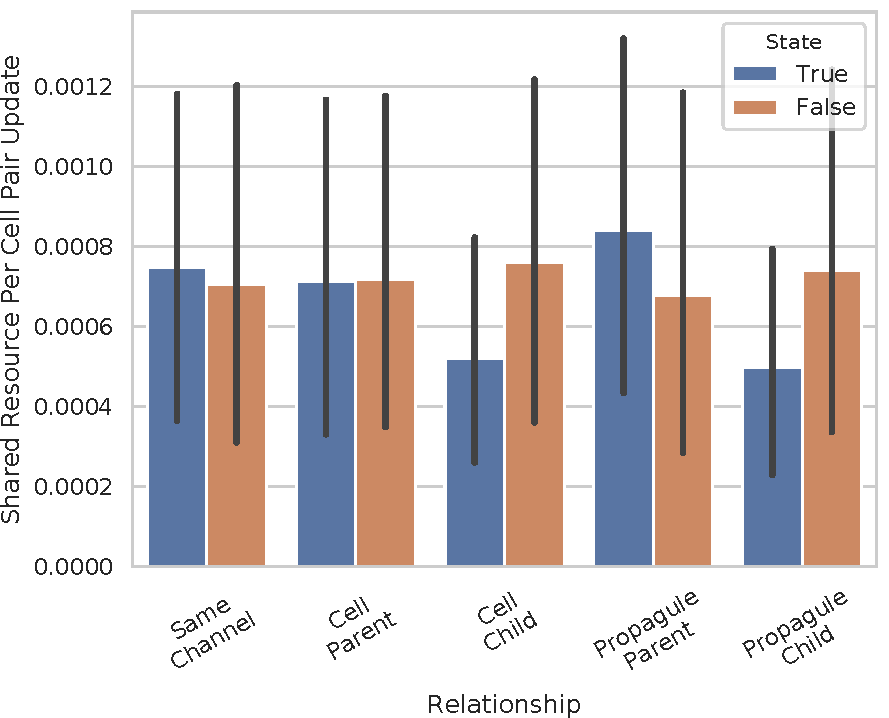
\includegraphics[width=\linewidth]{title=resource_contributed+treat=wave-small__mut-d_high+_data_hathash_hash=0508b355e6755132+_script_fullcat_hash=064800f3ddff6753+_source_hash=d53f428-clean+ext=}
\end{subfigure}
\hspace{1ex}
\begin{subfigure}[b]{0.1825\linewidth}
  \centering
  Mutational Load 5\\~\\
  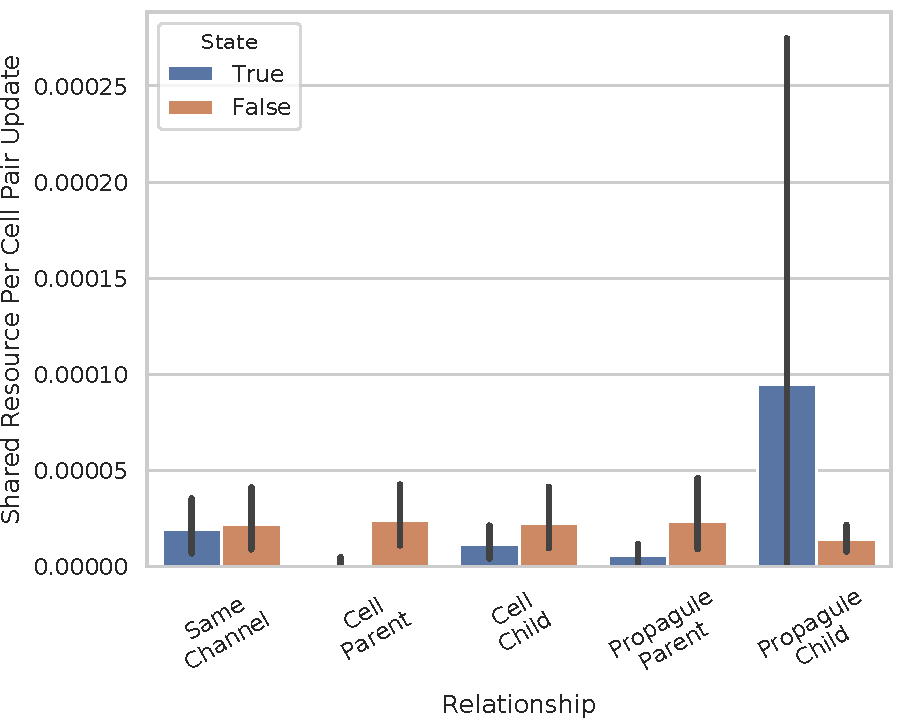
\includegraphics[width=\linewidth]{title=resource_contributed+treat=wave-small__mut-e_extreme+_data_hathash_hash=0b12a3f7b0d9143b+_script_fullcat_hash=064800f3ddff6753+_source_hash=d53f428-clean+ext=}
\end{subfigure}\\
\vspace{5ex}

\rotatebox{90}{~~~~~~Large Resource Wave}
\hspace{1ex}
\begin{subfigure}[b]{0.1825\linewidth}
  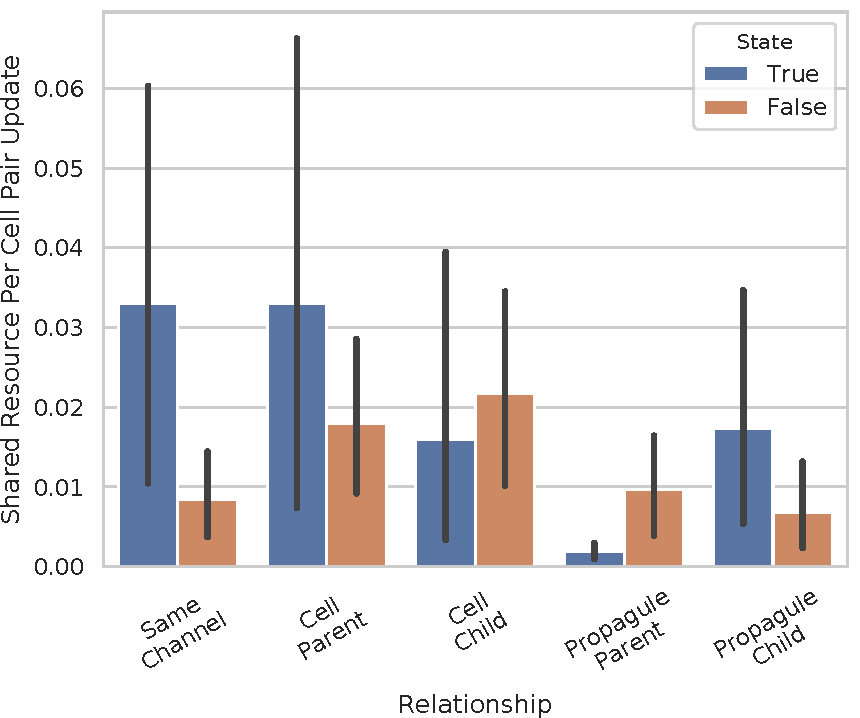
\includegraphics[width=\linewidth]{title=resource_contributed+treat=wave-big__mut-a_low+_data_hathash_hash=0687f354f3d94aaa+_script_fullcat_hash=064800f3ddff6753+_source_hash=d53f428-clean+ext=}
\end{subfigure}
\hspace{1ex}
\begin{subfigure}[b]{0.1825\linewidth}
  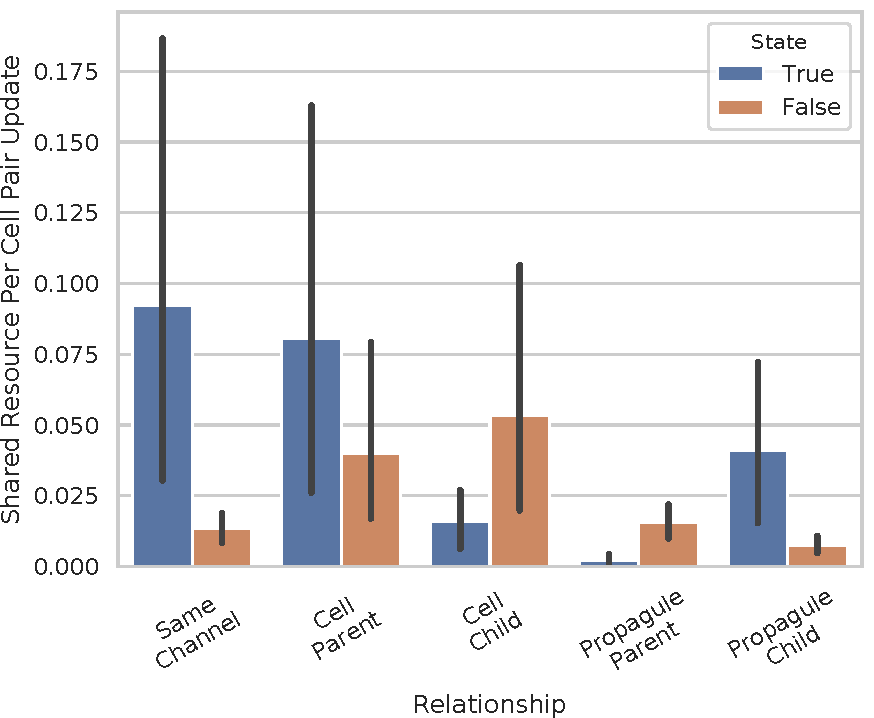
\includegraphics[width=\linewidth]{title=resource_contributed+treat=wave-big__mut-b_medlow+_data_hathash_hash=91d8a5c7499340cf+_script_fullcat_hash=064800f3ddff6753+_source_hash=d53f428-clean+ext=}
\end{subfigure}
\hspace{1ex}
\begin{subfigure}[b]{0.1825\linewidth}
  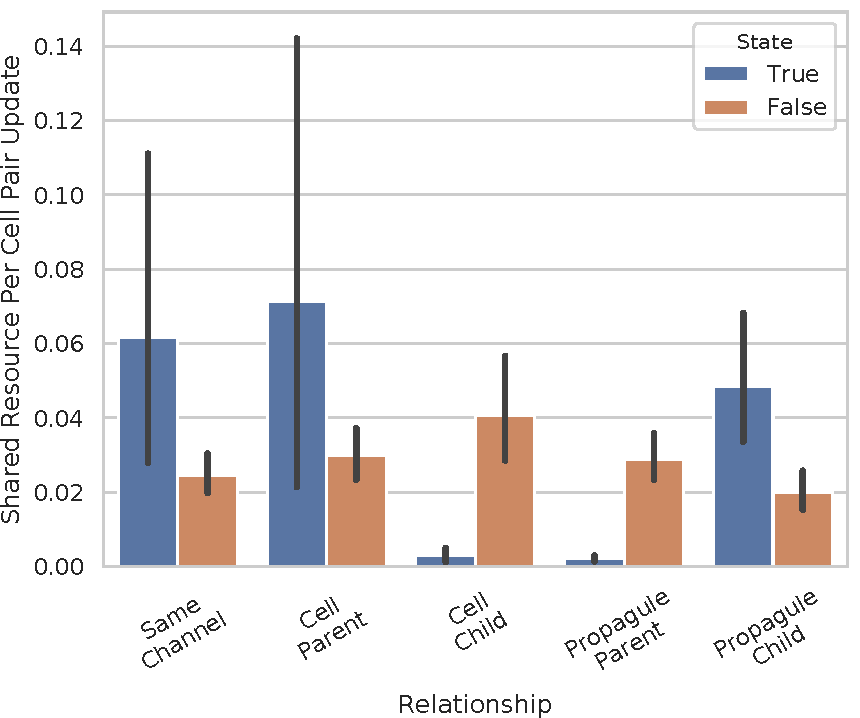
\includegraphics[width=\linewidth]{title=resource_contributed+treat=wave-big__mut-c_medhigh+_data_hathash_hash=9046a546605ce7d0+_script_fullcat_hash=064800f3ddff6753+_source_hash=d53f428-clean+ext=}
\end{subfigure}
\hspace{1ex}
\begin{subfigure}[b]{0.1825\linewidth}
  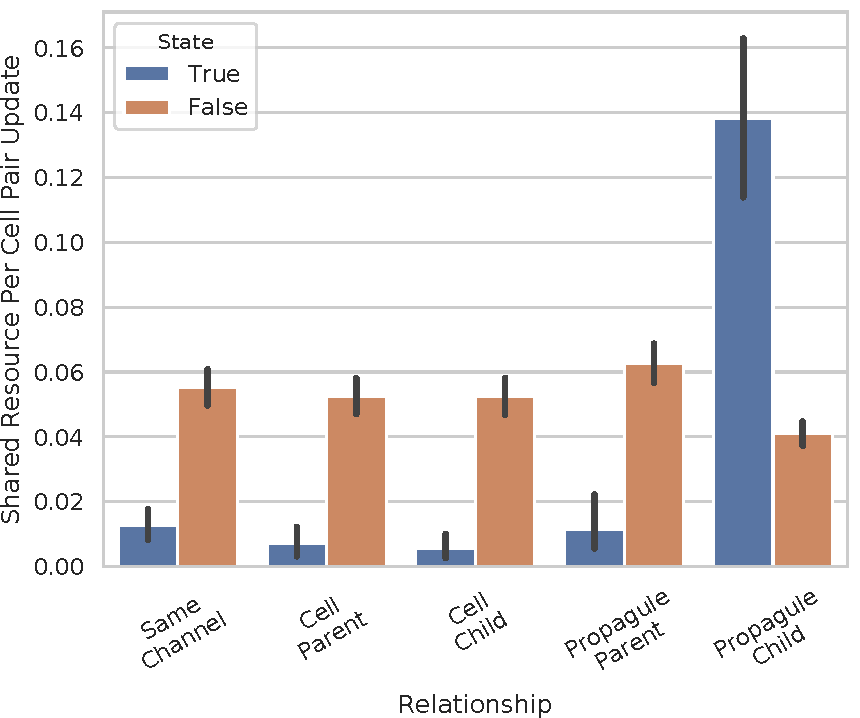
\includegraphics[width=\linewidth]{title=resource_contributed+treat=wave-big__mut-d_high+_data_hathash_hash=8c358ba0aef47998+_script_fullcat_hash=064800f3ddff6753+_source_hash=d53f428-clean+ext=}
\end{subfigure}
\hspace{1ex}
\begin{subfigure}[b]{0.1825\linewidth}
  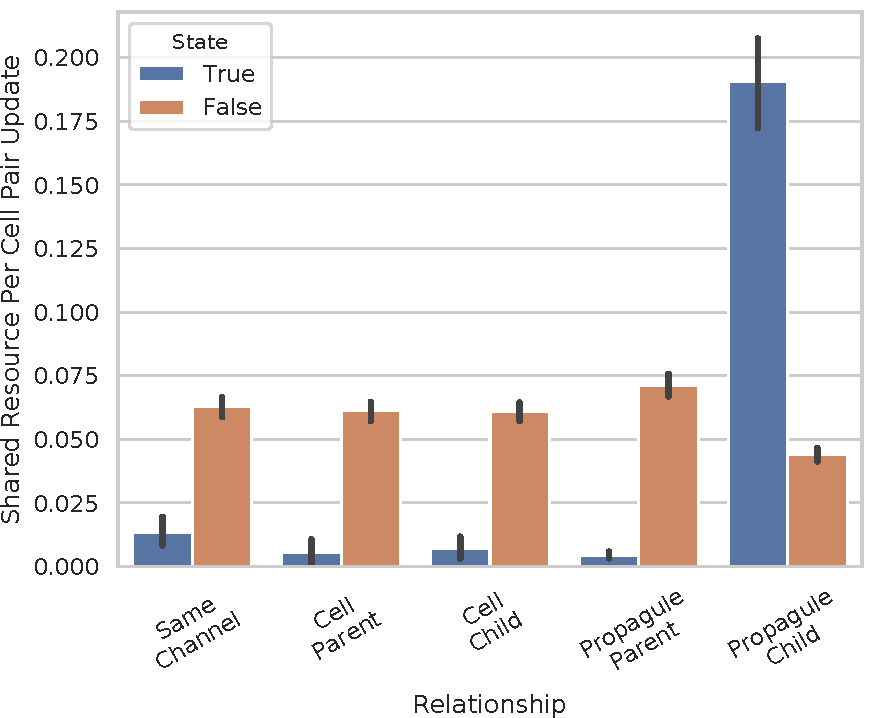
\includegraphics[width=\linewidth]{title=resource_contributed+treat=wave-big__mut-e_extreme+_data_hathash_hash=5e17f0d9addba523+_script_fullcat_hash=064800f3ddff6753+_source_hash=d53f428-clean+ext=}
\end{subfigure}\\
\vspace{5ex}
\caption{
Detailed audits of resource sharing phenotypes by treatment between updates 5000 and 50020.
Bar height represents the mean amount of resource transferred per update per neighboring pair of cells.
Each two-tone pair of bars compares cell pairs with a particular relationship to cell pairs without that relationship.
The ``Same Channel'' bar pair compares resource sharing between cell pairs with a common channel and cell pairs on different channels.
The ``Cell Parent'' bar pair compares the amount of resource shared from a cell to its cellular parent to the amount of resource shared from a cell to cells that are not its cellular parent.
The ``Cell Child'' bar pair compares the amount of resource shared from a cell to its cellular child to the amount of resource shared from a cell to cells that are not its cellular child.
For the next two relationships, consider a cell with channel ID $A$ that reproduces, producing a daughter cell with the new channel ID $B$.
Let the channel ID $C$ denote a channel ID that is unique from channel IDs $A$ and $B$.
The ``Propagule Parent'' bar pair compares the amount of resource shared from a cell to cells with the channel ID that its channel ID descends from (e.g., from cells with channel ID $B$ to cells with channel ID $A$) to the amount of resource shared to other cells that are not part of its same-channel network (e.g., to cells with channel ID $C$).
The ``Propagule Child'' bar pair compares the amount of resource shared from a cell to cells with a channel ID that descends from its channel ID (e.g., from cells with channel ID $A$ to cells with channel ID $B$) to the amount of resource shared to other cells that are not part of its same-channel network (e.g., to cells with channel ID $C$).
Error bars represent 95\% confidence intervals.
}
\label{fig:resource_contributed_by_treat}
\end{center}
\end{sidewaysfigure*}


Figure \ref{fig:resource_contributed_by_treat}, which provides a more detailed look at resource sharing behavior under each treatment, helps to explain the observation of preferential resource sharing with other-channel neighbors.
At mutational load levels three, four, and five with large resource wave conditions, a cell preferentially shares resource with members of same-channel groups that descend from that cell's same-channel group ($p < 0.05$; non-overlapping 95\% confidence intervals).
To better understand, let's consider a hypothetical example: a cell with channel ID $A$ reproduces, producing a daughter cell with the new channel ID $B$.
Under the conditions in question, Figure \ref{fig:resource_contributed_by_treat} shows that cells in channel group $A$ tend to send resource to cells in channel group $B$.
This resource-sharing pattern between a parental same-channel group and a propagule same-channel group is analogous to offspring endowment behaviors commonly observed in biological systems (e.g., breastfeeding in mammals or nutritious endosperm in plant seeds).
In previous work with DISHTINY, we observed the evolution of propagule endowment behavior (which helps new same-channel groups grow a resource collection network large enough to be self-sufficient) in the context of cooperative same-channel groups \citep{moreno2018toward}.
However, it is surprising to observe this resource-sharing pattern under high mutational load, in the context (as discussed earlier) of antagonistic reproductive behavior among same-channel cells.
This situation might be analogized to a household where the parents distrust each other and fight bitterly but both nevertheless make contributions to the child's college savings plan.

As expected, at low mutational loads we observed resource sharing behavior between same-channel neighbors.
This behavior helps to grow and maintain same-channel groups, giving them a competitive advantage against groups that do not share resource.
Resource sharing is more robust to mutational load in large resource wave treatments, perhaps because it is more important to ensure the large same-channel resource collecting groups required under those conditions.

\begin{figure*}[!htbp]
\begin{center}

  \begin{subfigure}[b]{0.5\linewidth}
    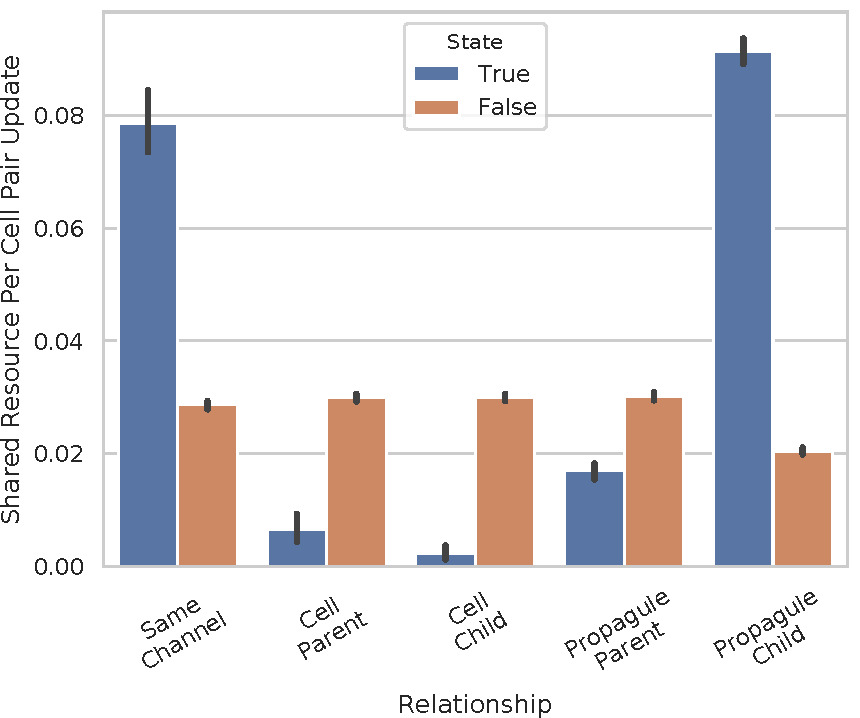
\includegraphics[width=\linewidth]{title=resource_contributed_start+treat=wave-big__mut-d_high+_data_hathash_hash=b9225de9509badc8+_script_fullcat_hash=064800f3ddff6753+_source_hash=d53f428-clean+ext=}
    \caption{Large Resource Wave, Mutational Load 4}
  \end{subfigure}

  \begin{subfigure}[b]{0.5\linewidth}
    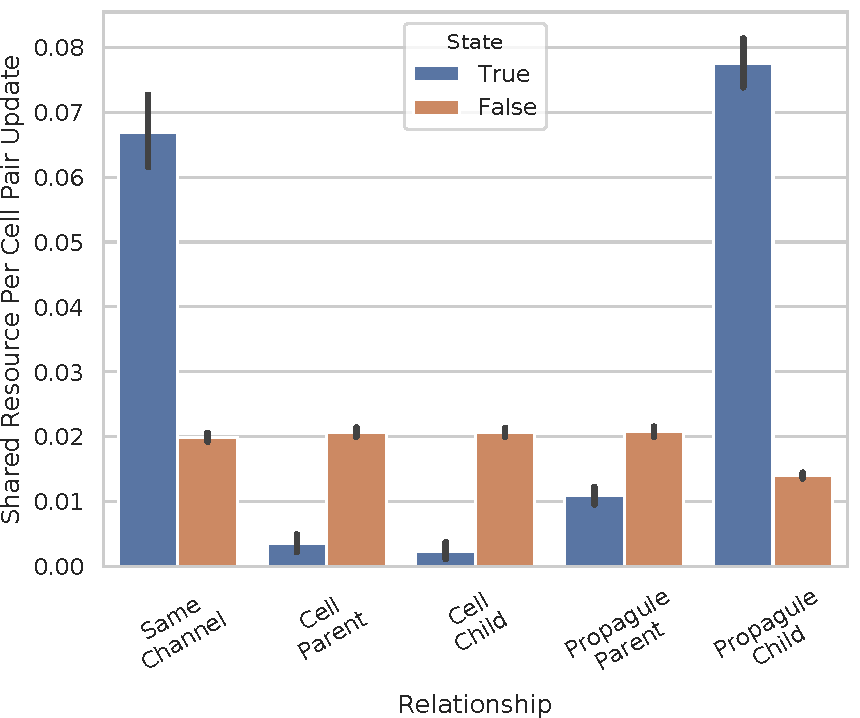
\includegraphics[width=\linewidth]{title=resource_contributed_start+treat=wave-big__mut-e_extreme+_data_hathash_hash=83586cb816dd102d+_script_fullcat_hash=064800f3ddff6753+_source_hash=d53f428-clean+ext=}
    \caption{Large Resource Wave, Mutational Load 5}
  \end{subfigure}

\caption{
Resource sharing phenotypes between updates 0 and 20 for high mutational load, large resource wave treatments.
Bar height represents the mean amount of resource transferred per update per neighboring pair of cells.
Each two-tone pair of bars compares cell pairs with a particular relationship to cell pairs without that relationship.
The ``Same Channel'' bar pair compares resource sharing between cell pairs with a common channel and cell pairs on different channels.
The ``Cell Parent'' bar pair compares the amount of resource shared from a cell to its cellular parent to the amount of resource shared from a cell to cells that are not its cellular parent.
The ``Cell Child'' bar pair compares the amount of resource shared from a cell to its cellular child to the amount of resource shared from a cell to cells that are not its cellular child.
For the next two relationships, consider a cell with channel ID $A$ that reproduces, producing a daughter cell with the new channel ID $B$.
Let the channel ID $C$ denote a channel ID that is unique from channel IDs $A$ and $B$.
The ``Propagule Parent'' bar pair compares the amount of resource shared from a cell to cells with the channel ID that its channel ID descends from (e.g., from cells with channel ID $B$ to cells with channel ID $A$) to the amount of resource shared to other cells that are not part of its same-channel network (e.g., to cells with channel ID $C$).
The ``Propagule Child'' bar pair compares the amount of resource shared from a cell to cells with a channel ID that descends from its channel ID (e.g., from cells with channel ID $A$ to cells with channel ID $B$) to the amount of resource shared to other cells that are not part of its same-channel network (e.g., to cells with channel ID $C$).
Error bars represent 95\% confidence intervals.
} \label{fig:resource_contributed_start}
\end{center}
\end{figure*}


The surprising observation of propagule endowment in antagonistic same-channel groups is likely an artifact of the small number of cellular generations elapsed in treatments with large resource wave size and high mutational load.
Figure \ref{fig:resource_contributed_start} shows the resource sharing behavior observed at the very beginning of the evolutionary run, between updates 0 through 20 for large resource wave treatments at mutational load levels four and five.
The genomes randomly seeded at the beginning of the evolutionary run exhibit significant same-channel and to-propagule resource sharing, likely induced by event triggers ``Neighbor's Channel ID Matches Mine'' and ``Neighbor's Channel ID Descends From Mine.''
As we saw in Figure \ref{fig:resource_contributed_by_treat}, by the end of these evolutionary runs the same-channel resource sharing behavior is gone but the to-propagule resource sharing remains.
From this data, whether to-propagule resource sharing remains after several cellular generations because it is advantageous or because it simply is not strongly detrimental enough to have been selected away yet remains uncertain.
Longer evolutionary runs where more cellular generations elapse under these treatments would help resolve this question.
